
%%% Local Variables: 
%%% mode: latex
%%% TeX-master: t
%%% End: 

\chapter{环结构在视网膜图像配准中的应用}
\label{cha:intro}


\section{视网膜图像配准研究现状}
\label{}

视网膜是人类的重要视觉器官,通过观察视网膜血管图像,医生能诊断和治疗眼底循环障碍疾病以及全身性疾病,比如青光眼、白内障、糖尿病等。但由于成像条件的限制,视网膜图像表现出中间亮、四周暗、对比度弱、有强噪声干扰的特点,可能会导致医生误诊。因此,通过图像处理与分析技术对视网膜图像进行质量改善、图像配准等自动分析,对疾病的诊断和治疗有着非常重要的价值。

视网膜配准技术是辅助眼科诊断和治疗的关键技术。视网膜血管图像通常是在不同时间或角度下获取的,包含有价值的时间与局部信息。通过视网膜配准技术,将多幅同一个个体的图像变换到同一幅图像中,就可以更加全面的显示视网膜特征,从而帮助医生进行比较和分析以选择合适的治疗方案。

目前,国内外有大量的视网膜图像配准相关的研究工作,主要可以分为两类:基于强度的视网膜图像配准与基于特征的视网膜图像配准\cite{oliveira2014medical}。

基于强度的视网膜配准方法通常基于互相关、相位相关、互信息\cite{penney1998comparison}等选择合适的相似性度量~\cite{Glocker02,Nunes03,Dreo04}。这些方法需要整合整幅图像的信息来完成配准,找到最佳的解决方案需要很大的计算成本。同时,基于强度的对准方法在图像质量较低或重叠区域较小的时候容易失败。这就刺激了基于特征的图像配准的发展。

基于特征的图像配准将对整个图像的分析转化为对图像特征的分析\cite{dingnan},因此,图像特征的选取是基于特征的方法中的关键问题。分叉点是视网膜血管的显著特征,大多数基于特征的图像配准把分叉点特征作为主要特征来进行特征匹配。Zana和Klein\cite{zana1999multimodal}利用分叉点及其周围的血管方向来做配准。Can和Stewart\cite{can2002feature}提出基于分叉点和交叉点的分层算法,能够在一定程度上减少特征错配。2003年,这一思想又进行了进一步的扩充,逐渐发展为双引导的迭代最近点算法\cite{stewart2003dual},它利用一种从简单到复杂,从局部到全局的策略最终确定最优的变换模型。Lalibert\cite{laliberte2003registration}等提出利用血管分叉点作为控制点来估计变换模型并利用了像素级的融合技术。Chanwimaluang\cite{chanwimaluang2006hybrid}等结合了基于区域和基于特征的方法,利用分叉点和交叉点来进行配准。Perez-Rovira\cite{perez2012rerbee}等提出了REES方法,利用分叉点和血管段来配准。这些方法很大程度上取决于单个分叉点的分支角度,但角度信息的精度不高容易引起分叉点错配,从而导致配准的失败。

与上述方法相比,基于结构的配准方法更容易克服错配的情况。Chen\cite{chen2011retinal,chen2015retinal}等人提出了基于分叉结构的配准方法,分叉结构由一个主分叉点和与它相连的三个相邻分叉点组成,归一化的分支角度和长度作为特征向量,一定程度上解决了错配的难题。Shen\cite{shen2012blood}等人扩展了基于分叉结构的配准方法,利用局部的精细配准来纠正配准精度。然而,若是血管树十分复杂,分叉结构特征仍然不够独特和可靠,因为复杂的血管树会使得匹配的血管丢失。

鉴于此,我们提出了基于环结构特征的从全局到局部的视网膜图像配准方法。环结构由血管分叉点和交叉点及与它们相连的血管组成。这一特征对于视网膜血管来说更加唯一和可靠,故它同样可应用于其他的领域,比如视网膜识别等。为了克服对视网膜分割结果的依赖性,我们采用多小波核多层分解方法,从而产生多尺度的血管树。不同尺度的血管树所代表的分割的精细程度不同。然后我们提出了动态路径移动算法来提取由多个不同数量的分叉点组成的多环特征,归一化的分支角度和长度来作为特征向量,采用相似性度量来进行全局初次配准。对于远离匹配特征的区域,我们采用局部分叉点信息来纠正配准精度。最后,我们采用骨架化对准精度来优化特征和尺度的选择,基本流程如图\ref{fig:framework}。
\begin{figure}[!ht]
  \centering
  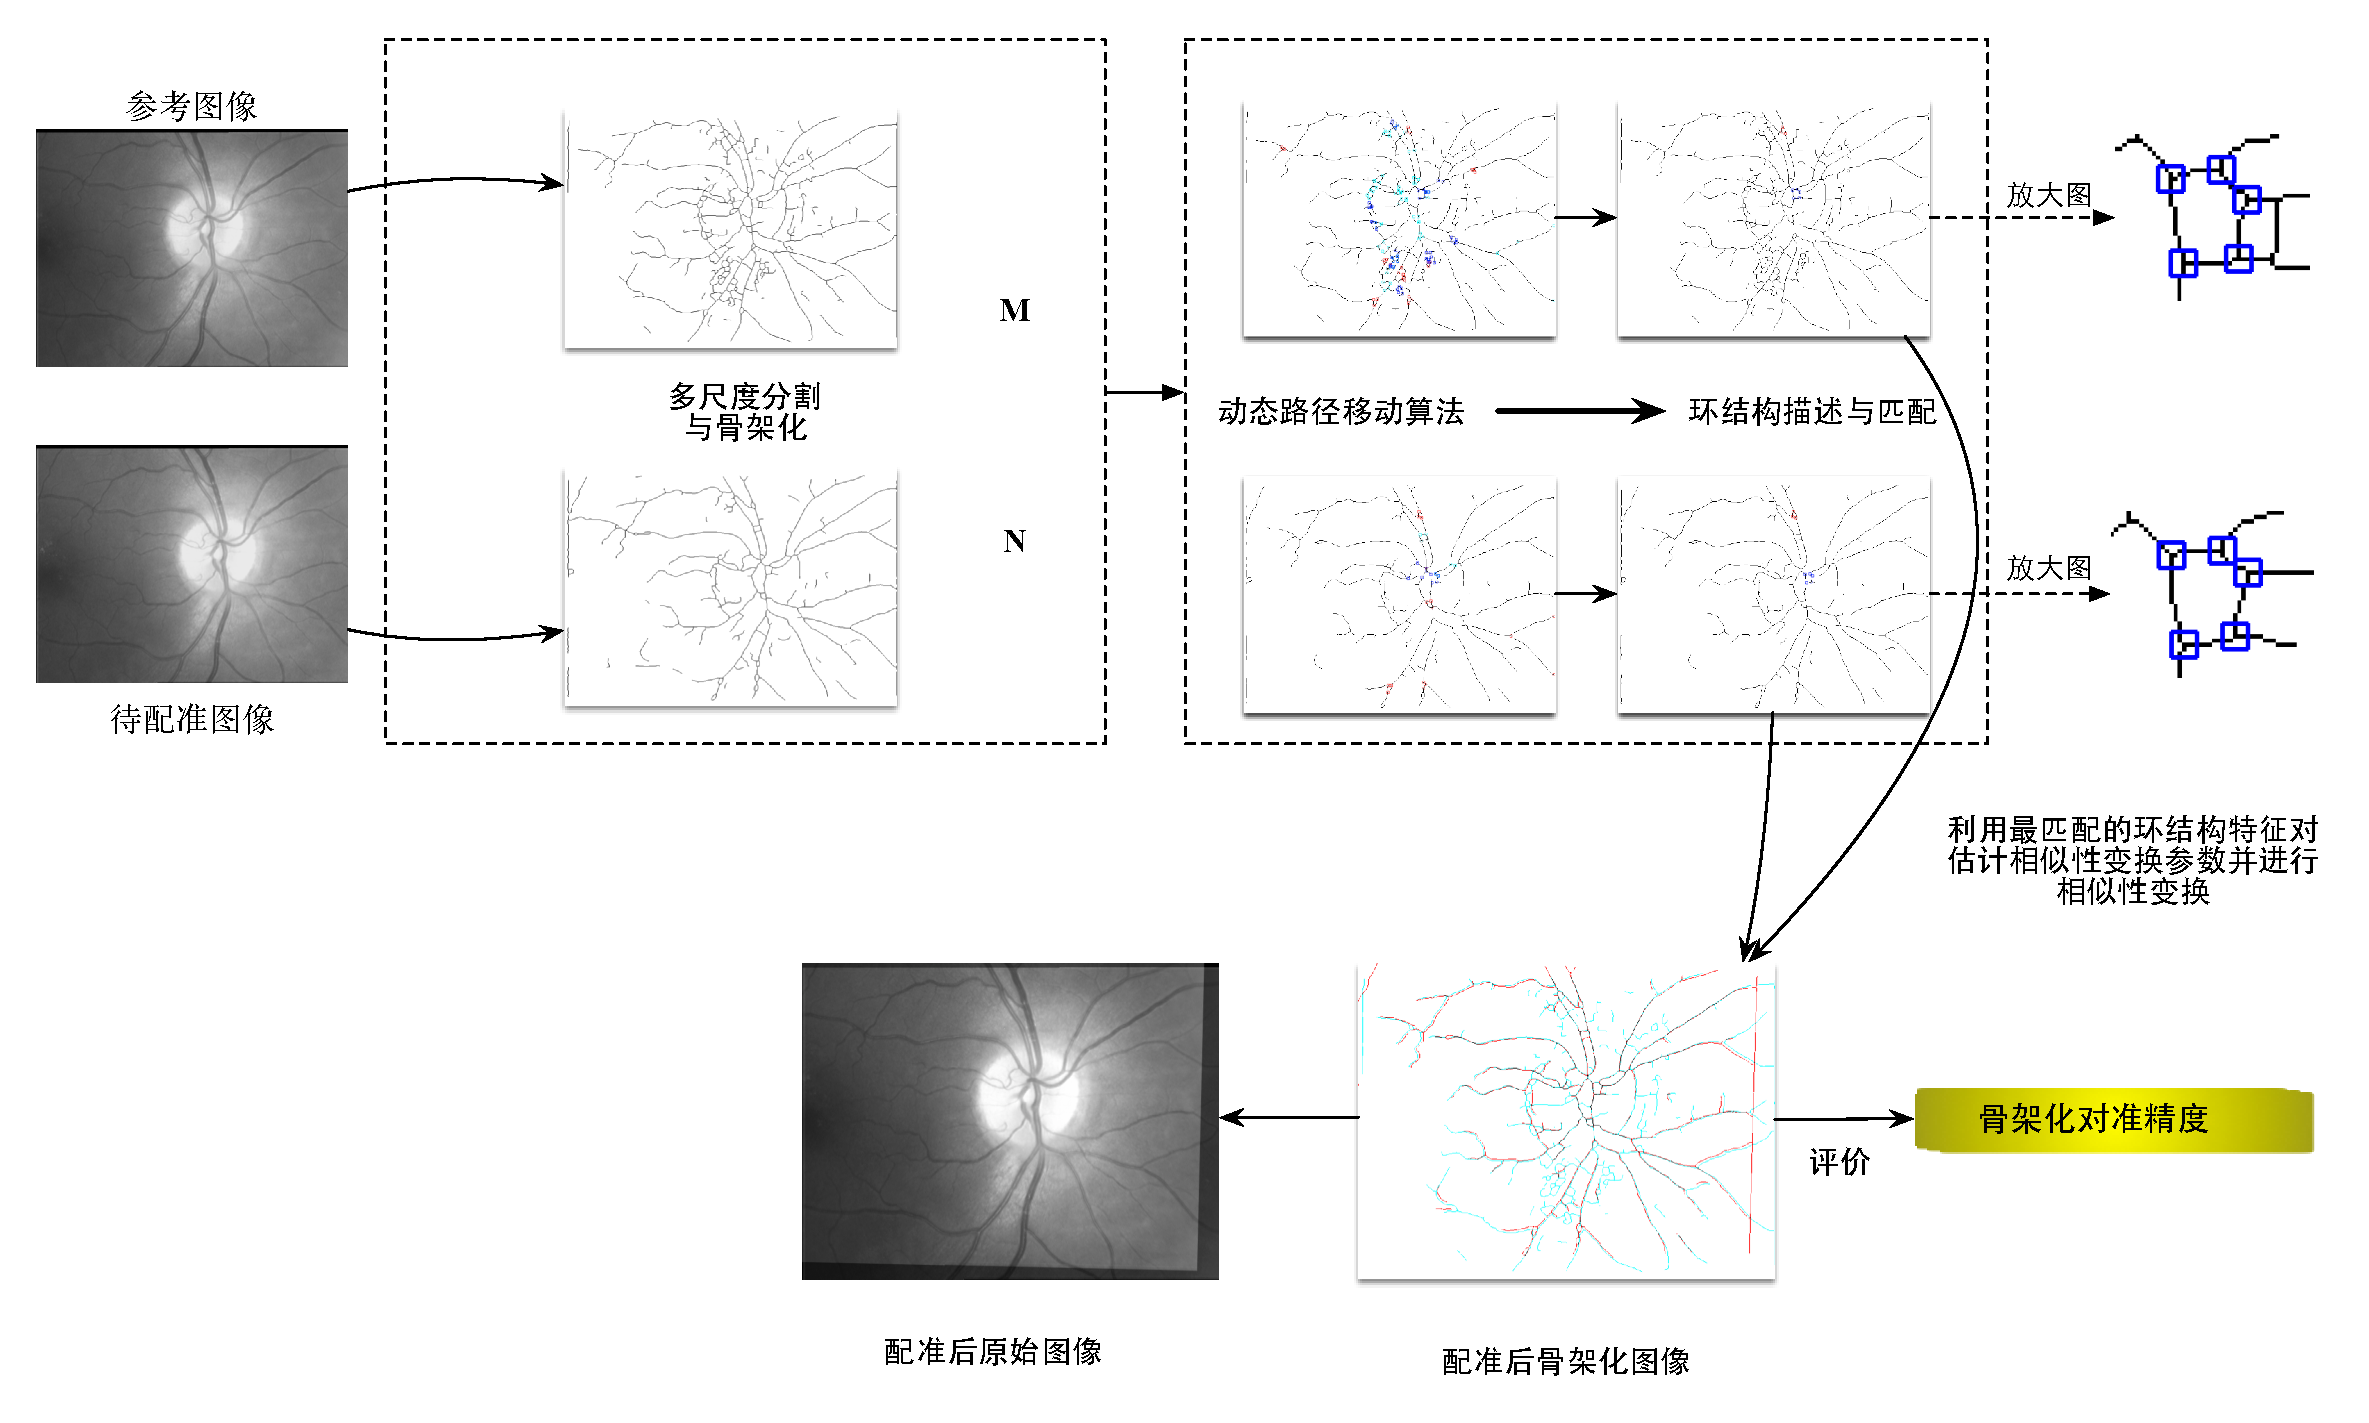
\includegraphics[width=1\textwidth]{figures/framework}
  \caption{基本框架}
  \label{fig:framework}
\end{figure}

\section{环结构全局配准}
\label{}
由第\ref{cha:cycle}章可知,采用多小波核多层分解方法,可以产生多尺度的血管树,为了确保配准的精度,我们选择了14个尺度的血管树,分别提取每个血管树中的环结构,描述成特征向量。这样,一幅图像则有14组特征向量。

视网膜图像配准是指将不同角度和时间获取的两幅同一个个体的图像变换到一幅图像中。两幅图像进行配准,即是$14 \time 14$组特征向量之间的匹配。我们采用相似性度量来寻找两幅图像特征向量之间的匹配对。

\subsubsection{相似性度量}
\label{cha:similarity}

假设参考图像的某一尺度与待配准图像的某一尺度分别有$m$和$n$组环结构特征,则他们之间的相似性测度为
\begin{align}
D_{pq} = mean(|V_p-W_q|), p = 1, 2, \ldots, m; q = 1, 2, \ldots, n
\end{align}
其中,$V_p$和$W_j$分别表示参考图像和待配准图像的第$p$个和第$q$个环结构。相似性测度越小,说明两个环结构越相似。为了保证最小的相似性测度相对应的环特征结构是匹配正确的,我们选择一个固定阈值来确保准确性,若最小测度仍大于这个阈值,我们认为这对环结构仍是不匹配的。

通过观察发现,视网膜血管图中,由三个分叉点、四个分叉点、五个分叉点组成的环居多,为了减小算法的复杂性,我们只选择三点环、四点环、五点环来作为特征。因此,相似性度量只在同种类型的环之间进行计算,得到最匹配的环结构。这种方法虽然可能丢失一些特征,但更能保证匹配的准确性且减小算法的复杂性。

\subsubsection{相似性变换}
\label{}

要使一幅图像变换到另一幅图像中,就要采用几何变换模型进行变换。几何变换模型是指坐标空间或图像 的像素值转换到另一个坐标空间或像素值的变换。常见的变换方式有平移、缩放、旋转、翻转、转置等。常用的空间变换模型有相似性变换、仿射变换、二次多项式变换等。

\begin{enumerate}
\item 平移,是指在一个平面内,将一个图像上的所有点都按照某个方向做相同距离的移动。平移不会改变图像的大小和形状。图像经过平移,对应角相等、对应线段相等、对应点所连的线段相等。它可视为同一个向量加到每个点上或将坐标系统的中心移动一定距离的结果。平移的方向不限于水平,也可为其它方向。设$(x_0,y_0)$是原图像上的一点,若将该图像沿水平方向平移tx,垂直方向平移ty,若平移后的坐标变为$(x_1,y_1)$,则其变换公式为:
\begin{align}
\left[ \begin{array}{c}
x_1 \\
y_1 \\
1   
\end{array} \right]
=
\left[ \begin{array}{ccc}
1 & 0 & tx \\
0 & 1 & ty \\
0 & 0 & 1
\end{array} \right]
\left[ \begin{array}{c}
x_0 \\
y_0 \\
1
\end{array} \right]
\end{align}
\item 在平面内,把一个图像绕一个定点沿某个方向转动一个角度,这样的变换叫做旋转。设$(x_0,y_0)$是原图像上的一点,若绕(0, 0)点旋转$\theta$角后,坐标变为$(x_1,y_1)$,则其变换矩阵为:
\begin{align}
\left[ \begin{array}{c}
x_1 \\
y_1 \\
1   
\end{array} \right]
=
\left[ \begin{array}{ccc}
cos\theta & sin\theta & 0 \\
-sin\theta & cos\theta & 0 \\
0 & 0 & 1
\end{array} \right]
\left[ \begin{array}{c}
x_0 \\
y_0 \\
1
\end{array} \right]
\end{align}
\item 缩放,即图像按一定的比例进行一定程度的放大或缩小。设图像在x轴方向的缩放比例为fx,在y轴方向的缩放比例为fy,则原图像中点$(x_0, y_0)$经缩放后的坐标变为$(x_1, y_1)$,则其变换矩阵为:

\begin{align}
\left[ \begin{array}{c}
x_1 \\
y_1 \\
1   
\end{array} \right]
=
\left[ \begin{array}{ccc}
fx & 0 & 0 \\
0 & fy & 0 \\
0 & 0 & 1
\end{array} \right]
\left[ \begin{array}{c}
x_0 \\
y_0 \\
1
\end{array} \right]
\end{align}
\item 由一个图像改变为另一个图像,在改变过程中保持形状不变的变换叫做相似变换。相似变换不改变图像中每一个角的大小,任何相似变换可以分解为缩放、平移、旋转和翻转的组合。相似性变换可定义为:
\begin{align}
X&=xs\cos\varphi-ys\sin\varphi+a\\
Y&=xs\sin\varphi+ys\cos\varphi+b
\end{align}
$s$代表缩放尺度,$\varphi$表示旋转角度,$(a, b)$表示参考图像与待配准图像的平移变化。
\item 仿射变换是图像平移、旋转、缩放、翻转、错切的复合。仿射变换可以用表示为:
\begin{align}
T = \left[ \begin{array}{ccc}
1 & 0 & 0 \\
0 & 0 & 0 \\
a & b & 0
\end{array} \right]
\times
\left[ \begin{array}{ccc}
1 & 0 & 0 \\
0 & 0 & 0 \\
-x & y & 0
\end{array} \right]
\times
\left[ \begin{array}{ccc}
cos\varphi & sin\varphi & 0 \\
-sin\varphi & cos\varphi & 0 \\
0 & 0 & 0
\end{array} \right]
\times
\left[ \begin{array}{ccc}
1 & 0 & 0 \\
0 & 0 & 0 \\
c & d & 0
\end{array} \right]
\label{eq:affine}
\end{align}
其中,$(a, b)$为图像的水平垂直平移量,$\varphi$表示旋转角度,$(x, y)$表示参考图像中的坐标点,$(c, d)$为旋转后的中心坐标。

仿射变换有六个自由量,六个自由量与六个可以变换的参数相对应,于是,将式\ref{eq:affine}变换可得
\begin{align}
X = a_1x + a_2y + a_3, 
\qquad
Y = a_4x + a_5y + a_6
\end{align}
仿射变换的主要特征是保持直线平行性和像素点的共线性。比如在进行映射时,即第一幅图像上的直线映射到第二幅图像上也是直线,方向不发生变化,但长度可能发生变化。
\item 假设三位空间中$P=(X, Y, Z)^T$和$Q=(X_1,Y_1,Z_1)^T$分别表示两幅图像中相应点的空间坐标,则空间中二次变换模型坐标为:
\begin{align}
Z = A_1X^2 + A_2XY + A_3Y^2 + A_4X + A_5Y + A_6
\label{eq:twice-4}
\end{align}
空间中刚体变换模型为
\begin{align}
\left[ \begin{array}{c}
X_1\\
Y_1\\
Z_1
\end{array} \right]
=
\left[ \begin{array}{ccc}
r_{11} & r_{12} & r_{13} \\
r_{21} & r_{22} & r_{23} \\
r_{31} & r_{32} & r_{33}
\end{array} \right]
\left[ \begin{array}{c}
X \\
Y \\
Z
\end{array} \right]
+
\left[ \begin{array}{c}
t_x \\
t_y \\
t_z
\end{array} \right]
\label{eq:twice-1}
\end{align}
其中,$r_{ij}$为空间正交变换矩阵的参数,$(t_x, t_y, t_z)$为空间平移参数,图像二维平面与三维空间之间的转换公式为:
\begin{align}
\left[ \begin{array}{c}
X \\
Y 
\end{array} \right]
=
\left[ \begin{array}{c}
\frac{sx-c_x}{a_x} \\
\frac{sy-c_y}{a_y}
\end{array} \right]
\label{eq:twice-2}
\end{align}
\begin{align}
Z = a_1x^2 + a_2xy + a_3y^2 + a_4x + a_5y + a_6
\label{eq:twice-3}
\end{align}
其中,$(a_x, a_y)$为尺存参数,s为图像的缩放比例,$(c_x, c_y)$为图像中心点的坐标。

将\ref{eq:twice-1}、\ref{eq:twice-2}、\ref{eq:twice-3}代入\ref{eq:twice-4}得:
\begin{align}
\left[ \begin{array}{c}
X_1 \\
Y_1
\end{array} \right]
=
\left[ \begin{array}{c}
r_{11}\frac{sx-c_x}{a_x} + r_{12}\frac{sy-c_y}{a_y} + r_{13} \\
(a_1x^2 + a_2xy + a_3y^2 + a_4x + a_5y + a_6)\\
r_{21}\frac{sx-c_x}{a_x} + r_{22}\frac{sy-c_y}{a_y} + r_{23}\\
(a_1x^2 + a_2xy + a_3y^2 + a_4x + a_5y + a_6)
\end{array} \right]
\label{eq:twice-5}
\end{align}
将\ref{eq:twice-5}变换到二维平面,可得12个自由参数,分别用$\theta_1 \sim \theta_{12}$代替,可得:
\begin{align}
\left[ \begin{array}{c}
x_1 \\
y_1
\end{array} \right]
=
\left[ \begin{array}{cccccc}
\theta_{11} & \theta_{12} & \theta_{13} & \theta_{14} & \theta_{15} & \theta_{16} \\
\theta_{21} & \theta_{22} & \theta_{23} & \theta_{24} & \theta_{25} & \theta_{26} 
\end{array} \right]
\left[ \begin{array}{c}
x^2, xy, y^2, x, y, 1
\end{array} \right]^T
\end{align}
通常情况下,高阶多项式通常不用于实际应用,因为利用高阶多项式进行配准时,在远离特征区域的地方,可能会造成不必要的变形。一般来说,特征的数目要多于决定映射函数所需要的最小数量。映射函数的参数通过最小二乘拟合方法计算,所以,多项式使得在特征周围的最小平方误差最小。但这样的映射对于远离特征周围的区域并不适用。
\end{enumerate}

根据相似性变换、仿射变换与二次多项式变换的性质,结合环结构的特点,我们采用相似性变换模型,因为仿射变换加入了错切,能使环结构中的角度发生变形,从而改变了原来环结构的形状。

变换时选取的点集越多,求取的变换模型参数就会越准确。由第\ref{cha:similarity}节我们可知,使得相似性度量最小的三点环、四点环、五点环可用来做配准特征。组成三点环、四点环、五点环的分叉点数分别是3、4、5,这些点的坐标可用来进行相似性参数估计。为了提高配准的成功率,我分别采用三点环、四点环、五点环、三点及四点环、三点及五点环、四点及五点环、三点四点及五点环七种组合来进行配准。即参考图像的某一个尺度与待配准图像的某一尺度共有7个配准结果,14个分割尺度即有$14 \times 14 \times 7$个配准结果。

为了确保配准的精准度,我们不仅使用组成环的分叉点的坐标,也检测了与环相连的血管上的点或分叉点加入特征点集。基本流程如图\ref{fig:global}。
\begin{figure}[!ht]
  \centering
  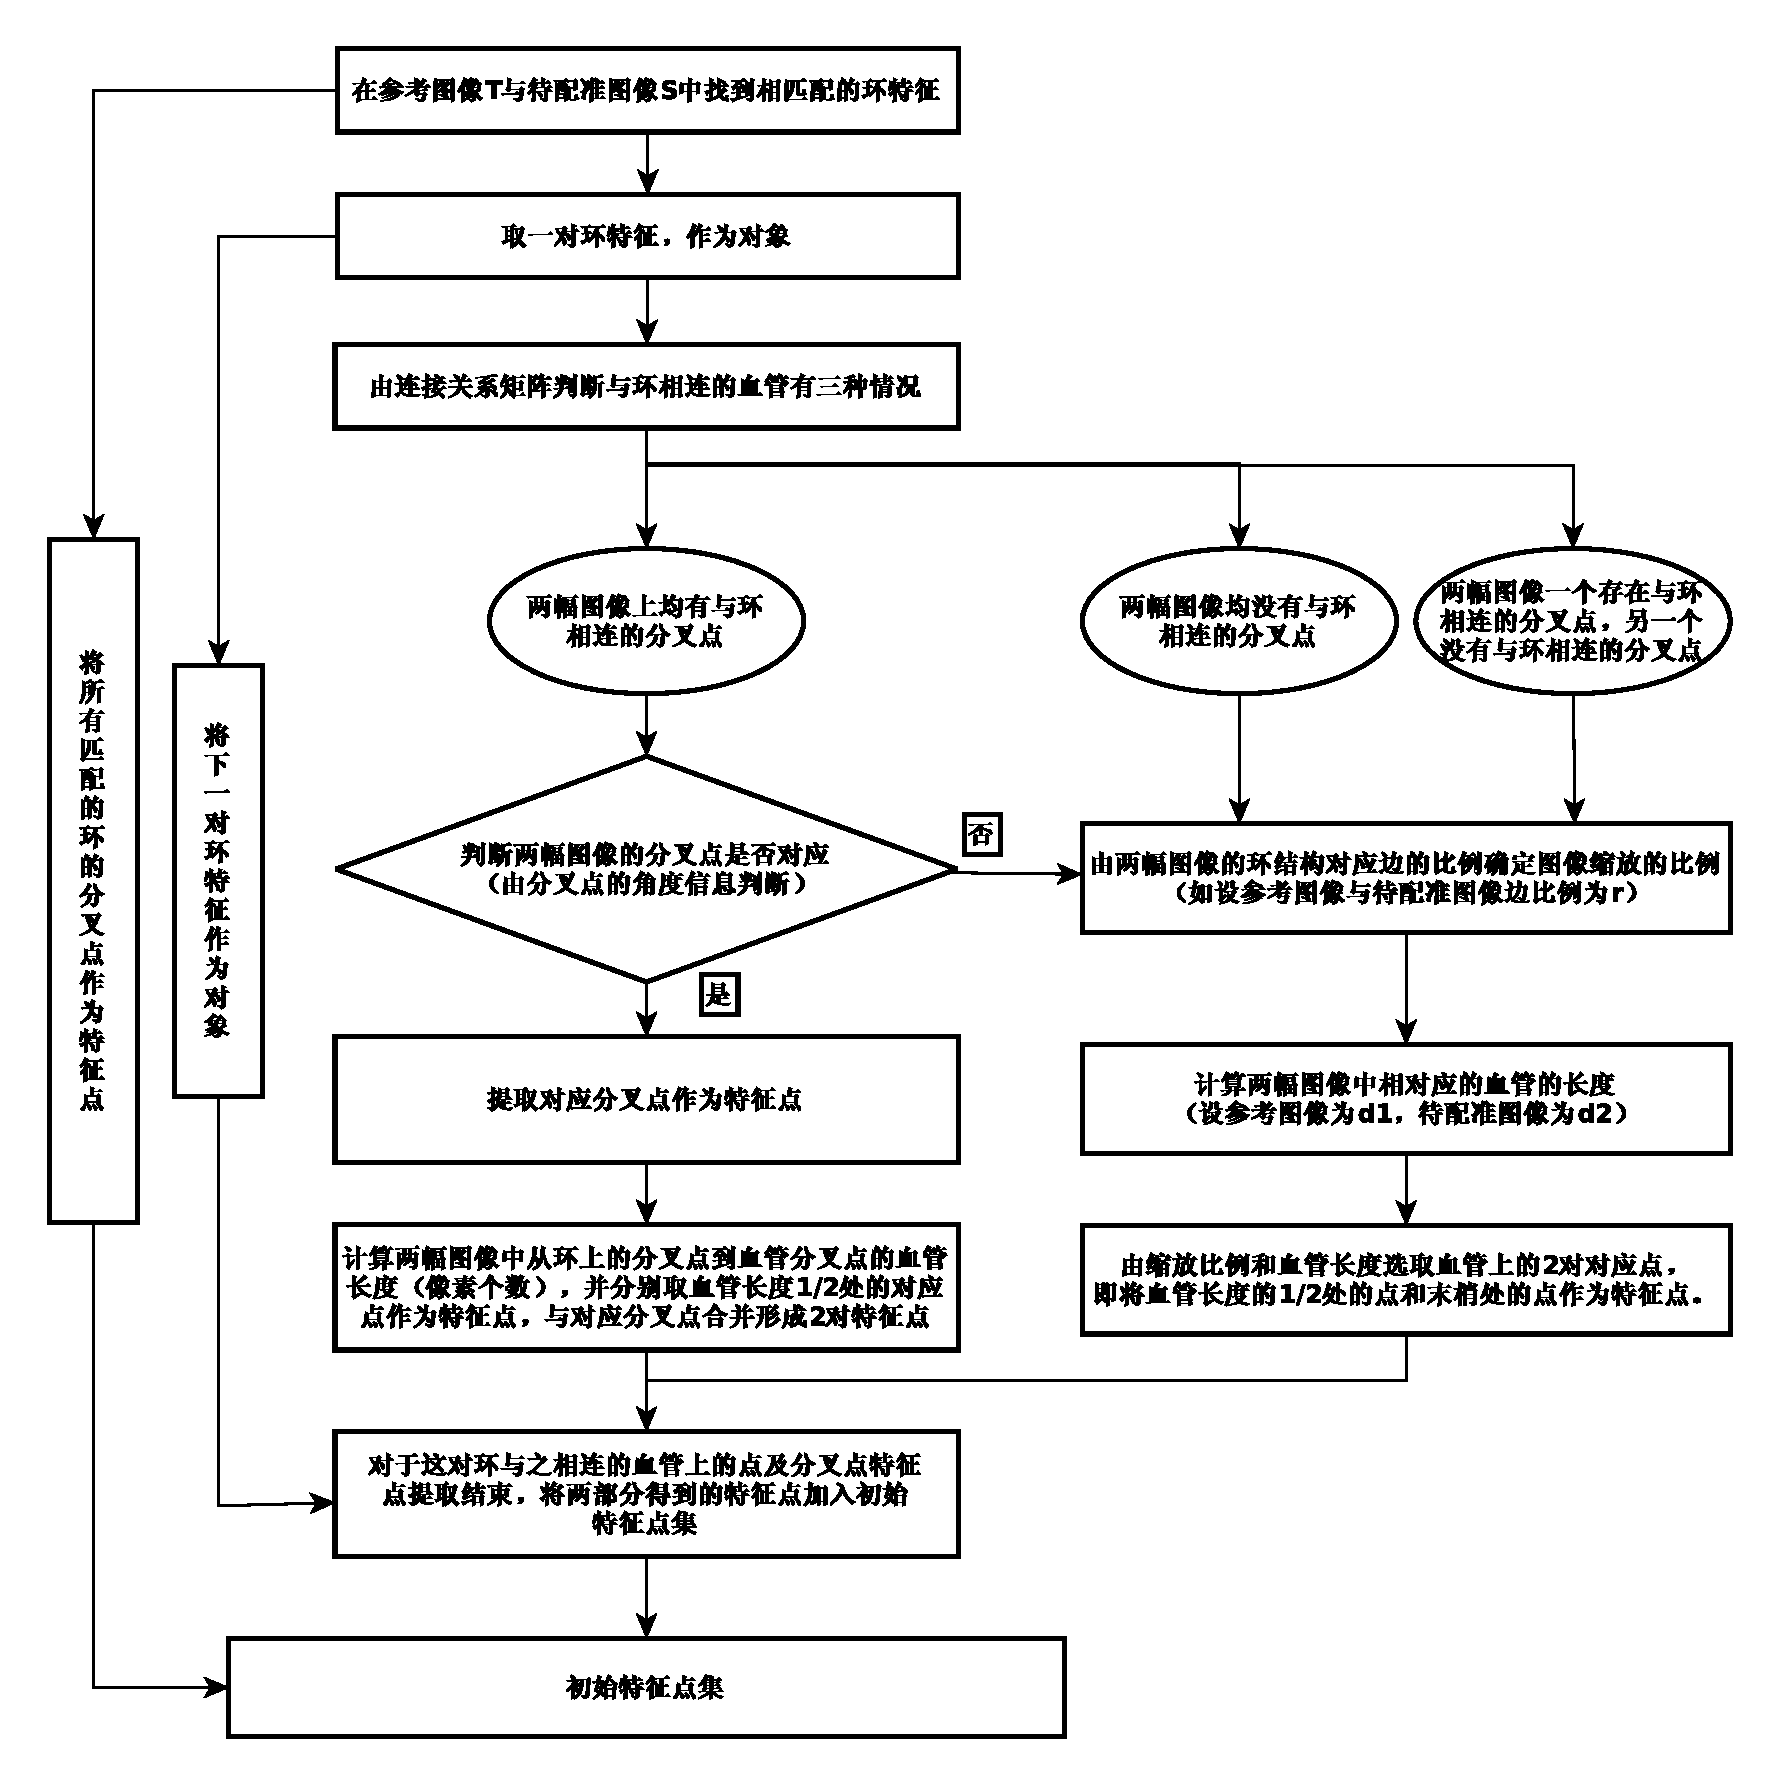
\includegraphics[width=1\textwidth]{figures/global}
  \caption{将与环相连的血管上的点加入特征点集}
  \label{fig:global}
\end{figure}

步骤为:
\begin{enumerate}
\item 从环上的一个分叉点开始,根据分叉点之间的连接关系,搜索与之相邻的除环以外的其他点。若参考图像与待配准图像上都存在这样的点,则转入第二步,否则转入第三步。
\item 判断这些与分叉点相邻的分叉点是否是相对应的,若是,则取血管的中心点与这个点加入特征点集,否则,则转入第三步。
\item 考虑到参考图像与待配准图像之间有可能有尺度变化,要通过计算相匹配的环结构中边长的比例关系来确定缩放尺度。从而根据缩放尺度找到相对应的与环相连的血管的中心点和端点,加入特征点集。

图\ref{fig:global points}显示了最匹配的环结构及与其相连的血管上的对应点。蓝色点为最匹配的环结构特征点对,红色点为与通过以上步骤得到的环相连的血管点。从图中可以看出,找到的点都是正确匹配的。
\end{enumerate}


\begin{figure}
\centering
  \begin{minipage}[b]{0.48\textwidth} 
      \centering 
      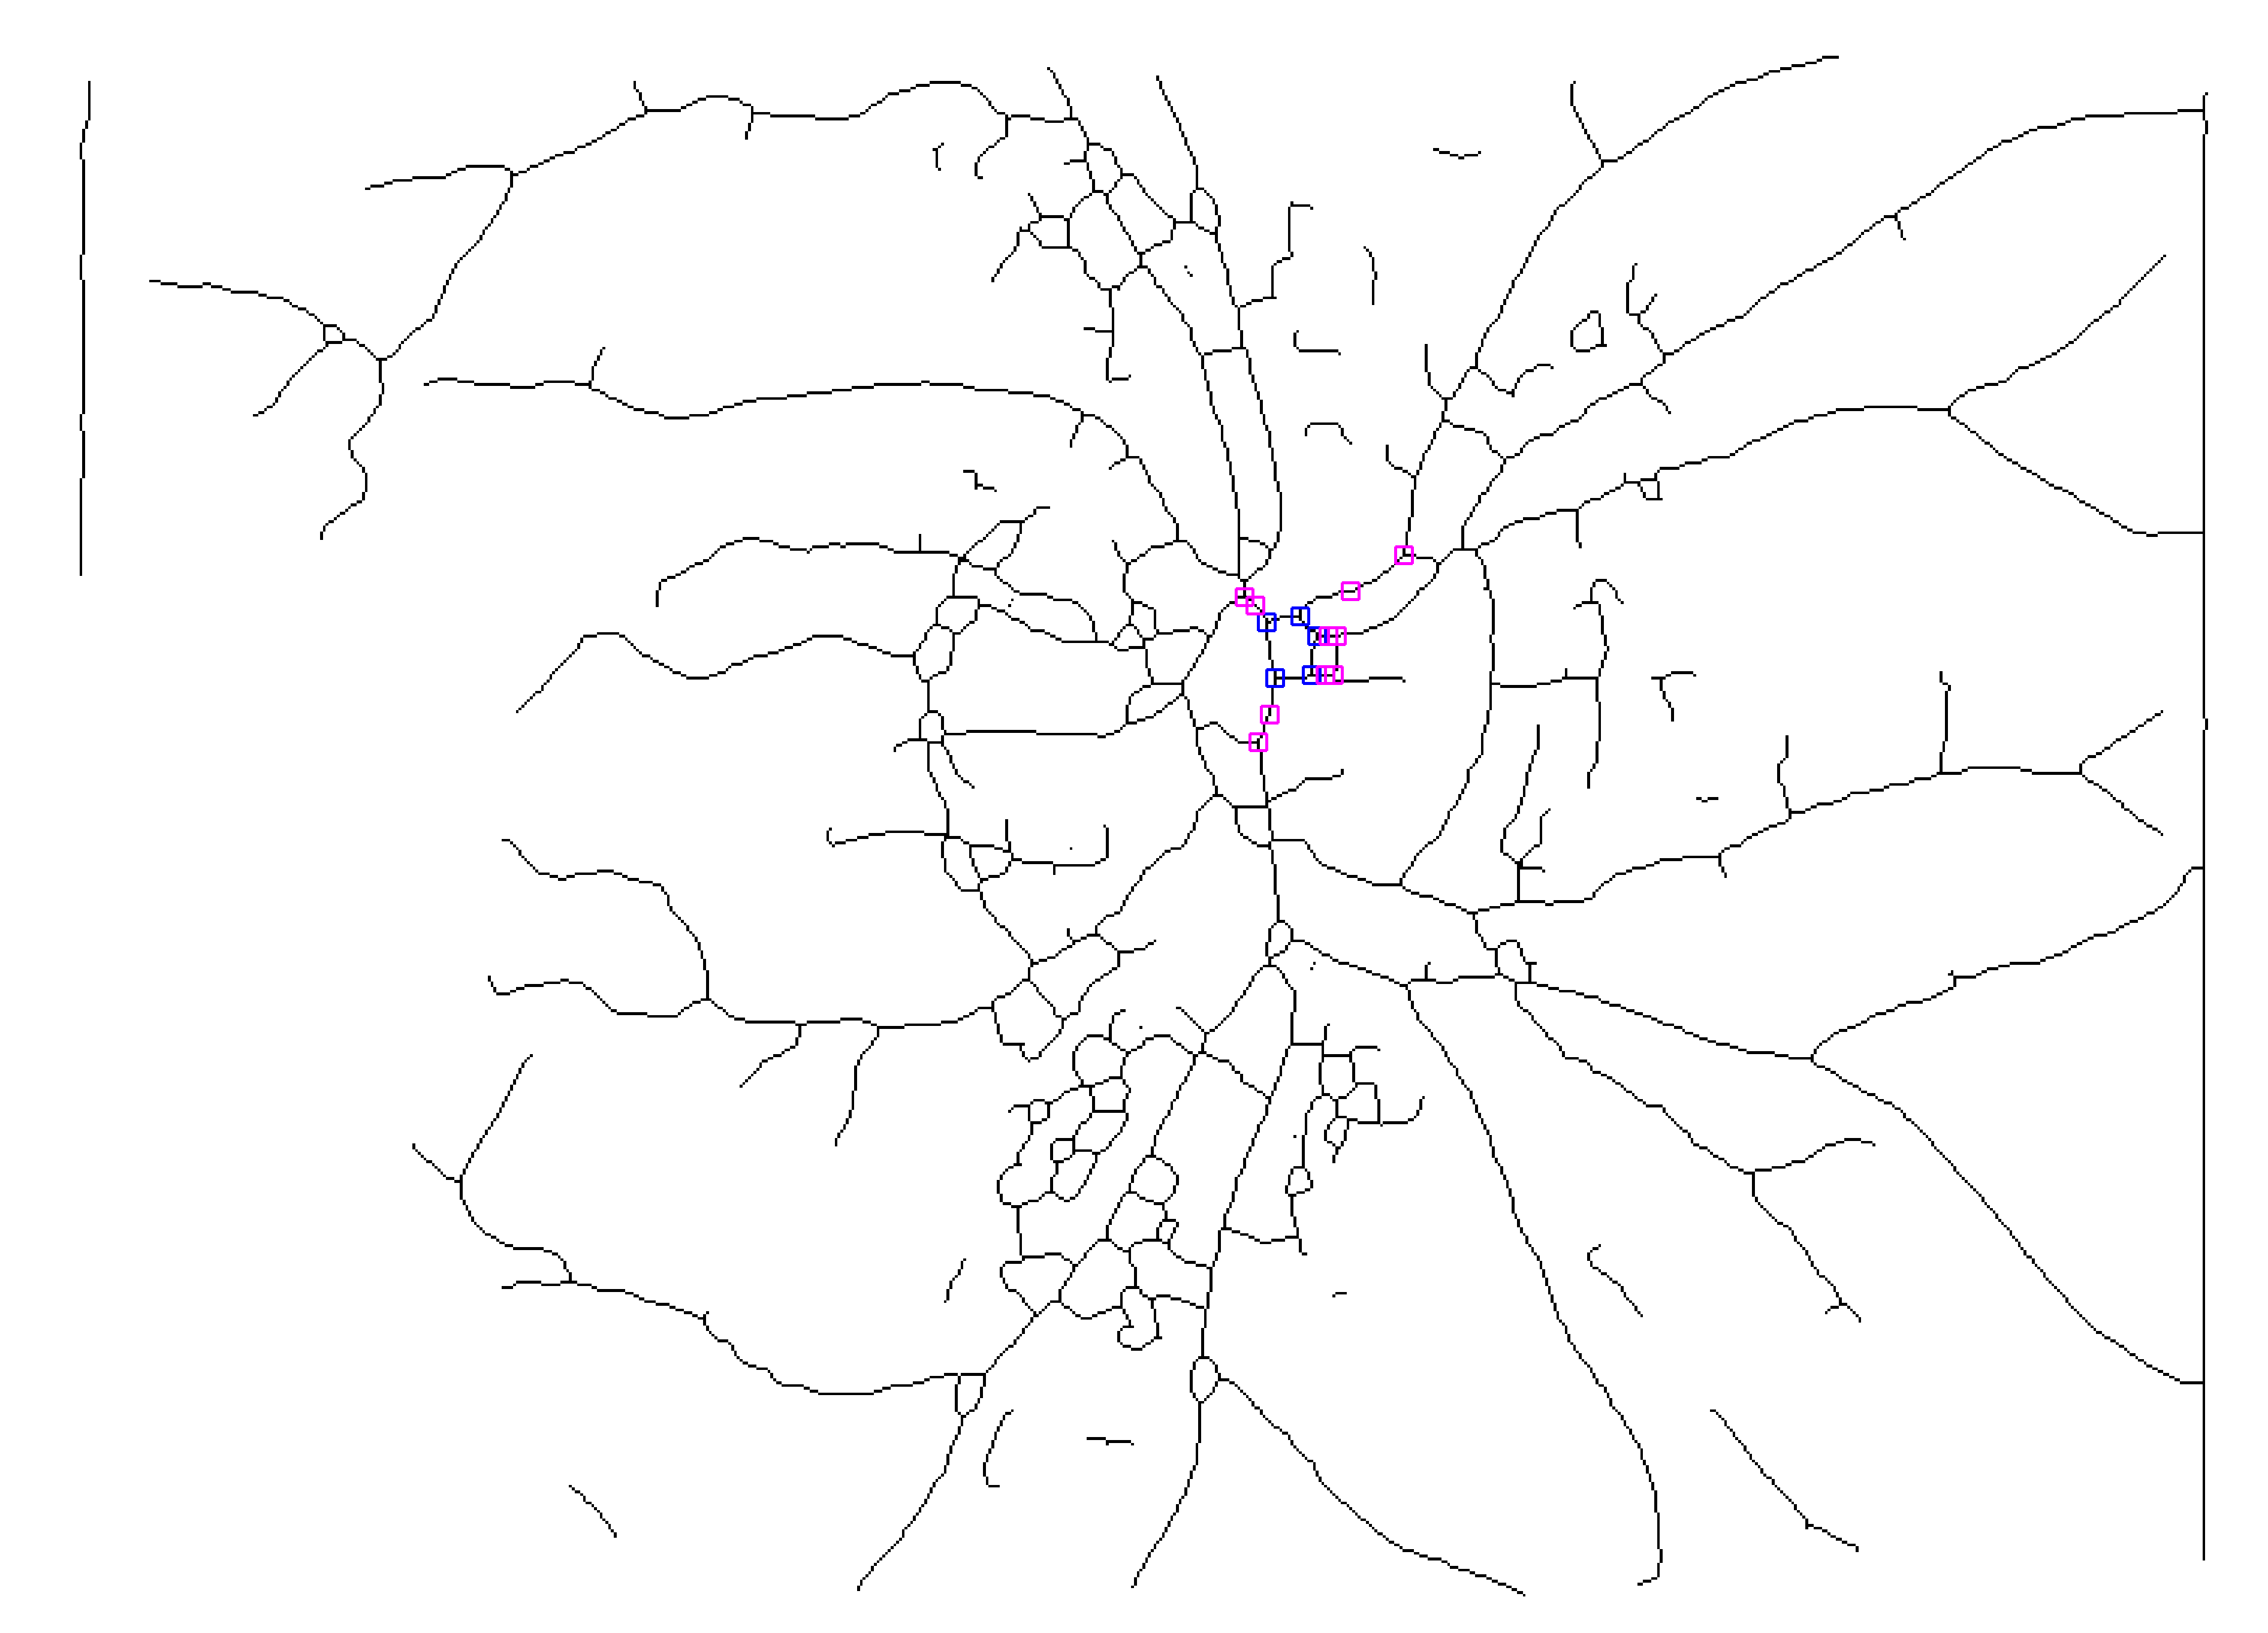
\includegraphics[width=6cm]{bw1-cycle-vessel}
        \centerline{(a) 参考图像}\medskip
    \end{minipage}
  \begin{minipage}[b]{0.48\textwidth}
    \centering
    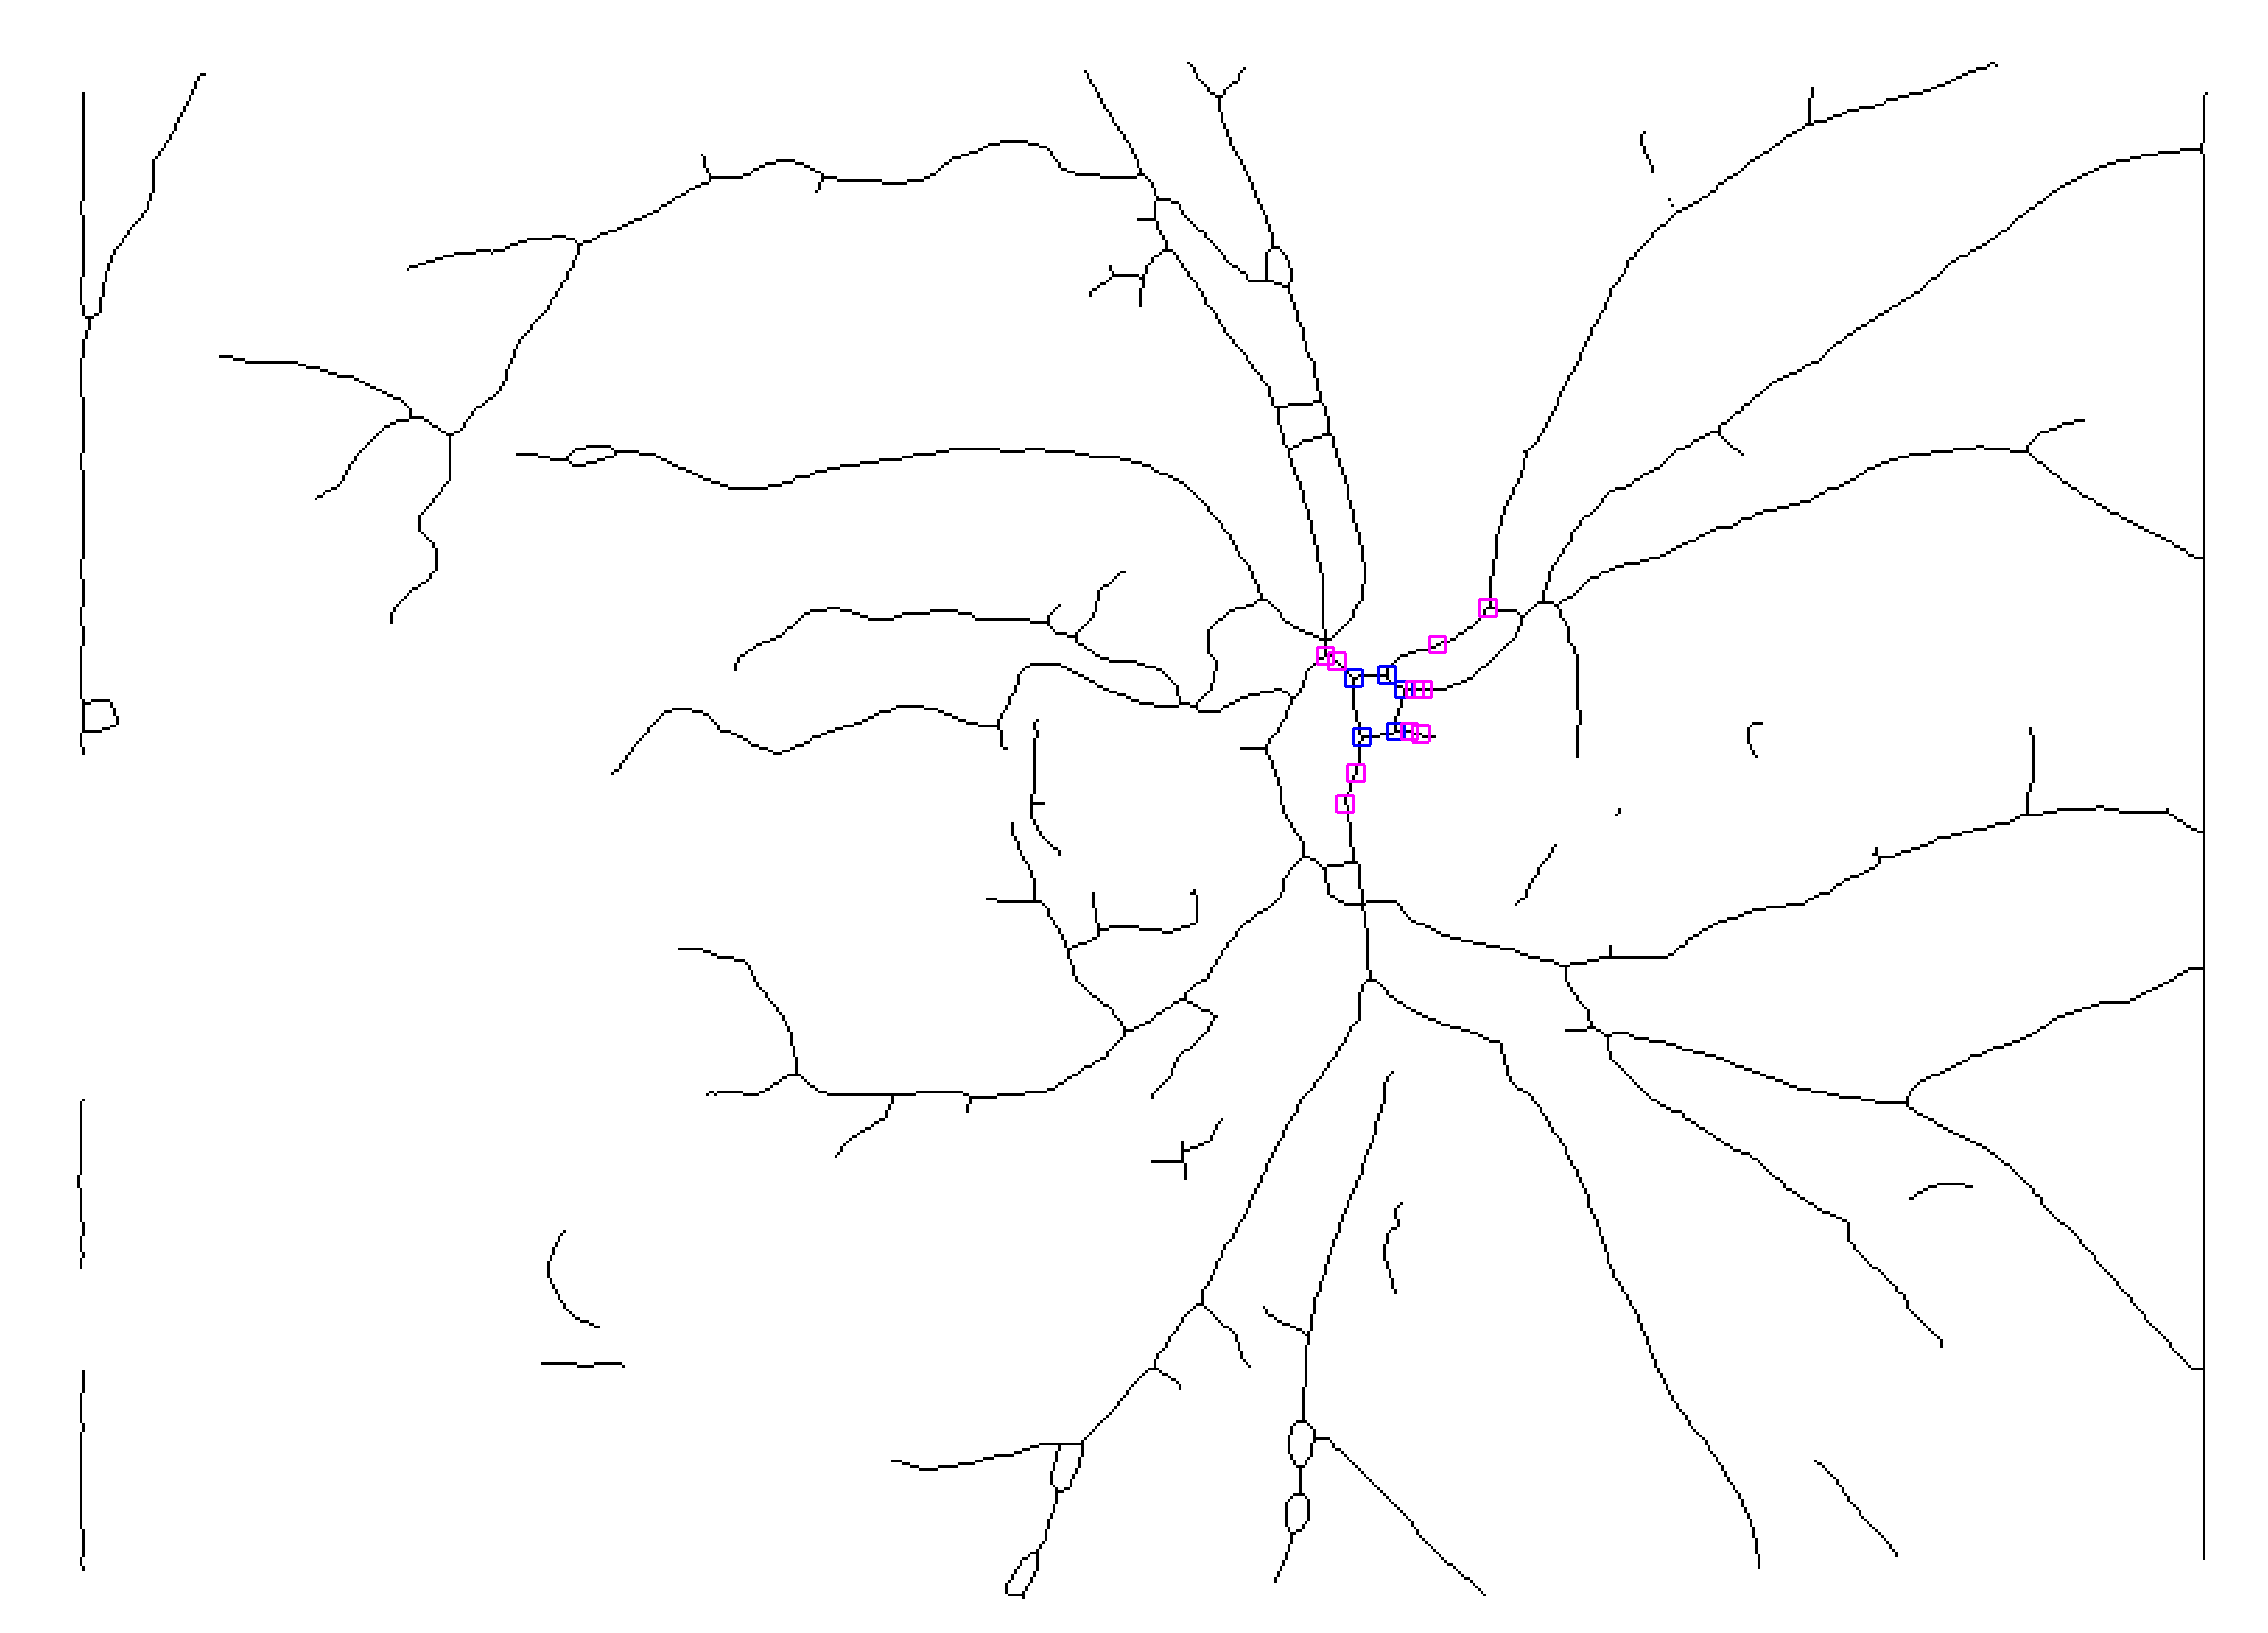
\includegraphics[width=6cm]{bw2-cycle-vessel}
      \centerline{(b) 待配准图像}\medskip
  \end{minipage}
\caption{相匹配的环结构及与其相连的血管上的对应点}
\label{fig:global points}
\end{figure}


根据特征点集中相对应的特征点的坐标进行相似性变换,于是,得到了全局初始配准结果,如图\ref{fig:global results}。


\begin{figure}
\centering
  \begin{minipage}[b]{0.48\textwidth} 
      \centering 
      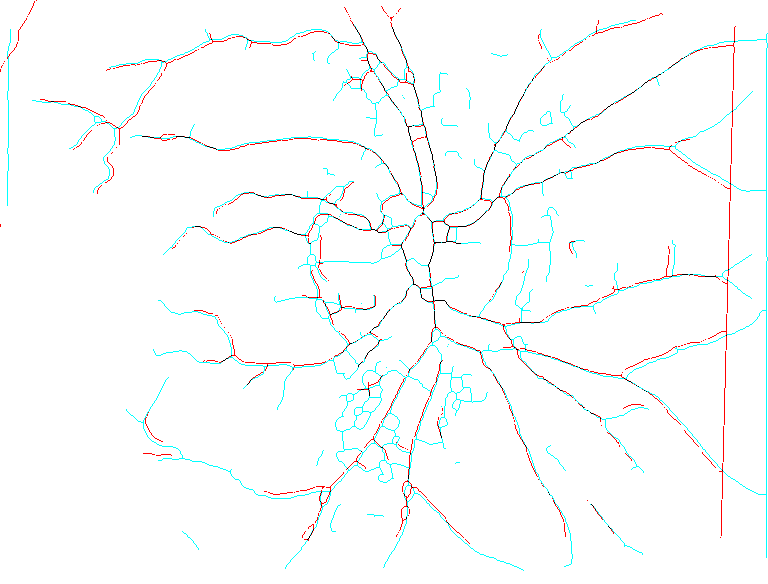
\includegraphics[width=6cm]{067-119-initial_reg}
        \centerline{(a) 骨架化配准结果}\medskip
    \end{minipage}
  \begin{minipage}[b]{0.48\textwidth}
    \centering
    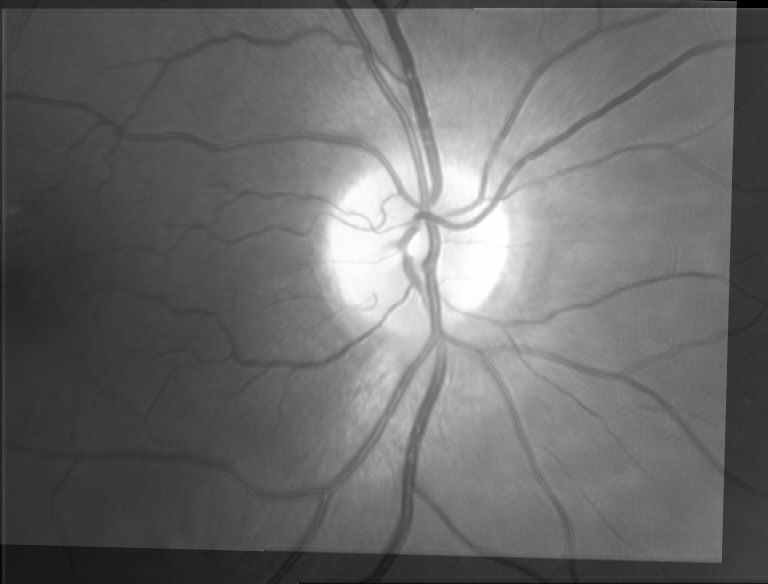
\includegraphics[width=6cm]{067-119-initial_result}
      \centerline{(b) 配准后的原图像}\medskip
  \end{minipage}
\caption{全局初始配准结果}
\label{fig:global results}
\end{figure}


\section{分叉点局部配准}
\label{}

由图\ref{fig:global results}可以看到,虽然使用环上的分叉点及与环相连的血管上的点能准确的进行配准,但仍不够鲁棒,远离这些特征点的区域会出现几个像素的偏差。因此,我们采用了一种从全局到局部的策略,即增加一些局部分叉点来纠正配不准的区域,以此来提高配准精度。配准流程图如图\ref{fig:local}。基本步骤为:
\begin{enumerate}
\item 检测参考图像中的所有分叉点,并分别以这些分叉点为中心,形成$5 \times 5$像素的区域。
\item 分别在配准后的图像中这些小区域内检测分叉点。根据分叉点的角度信息判断是否有与待配准图像中的分叉点相对应的分叉点。若有,则计算这两个分叉点之间的欧式距离。若欧式距离大于3,我们认为这一对对应点是没有配准的,那么应将其加入新的特征点集。否则,则认为没有未配准的对应点对。
\item 根据初始配准时相似性度量参数及对应点的坐标,将特征点集中配准后的图像中的分叉点映射回待配准图像中,将新的特征点集中的点变为参考图像与待配准图像中相对应的分叉点。
\item 将新的特征点集与初始特征点集合并,形成最终的特征点集。重新采用相似性变换进行第二次配准,得到经过局部修正的最终的配准结果。
\end{enumerate}
图\ref{fig:final-results}给出了两个例子,显示了全局与局部配准结果。从图中我们可以看出,在全局初始配准中未配准的血管经过局部配准后得到了纠正。
\begin{figure}[!ht]
  \centering
  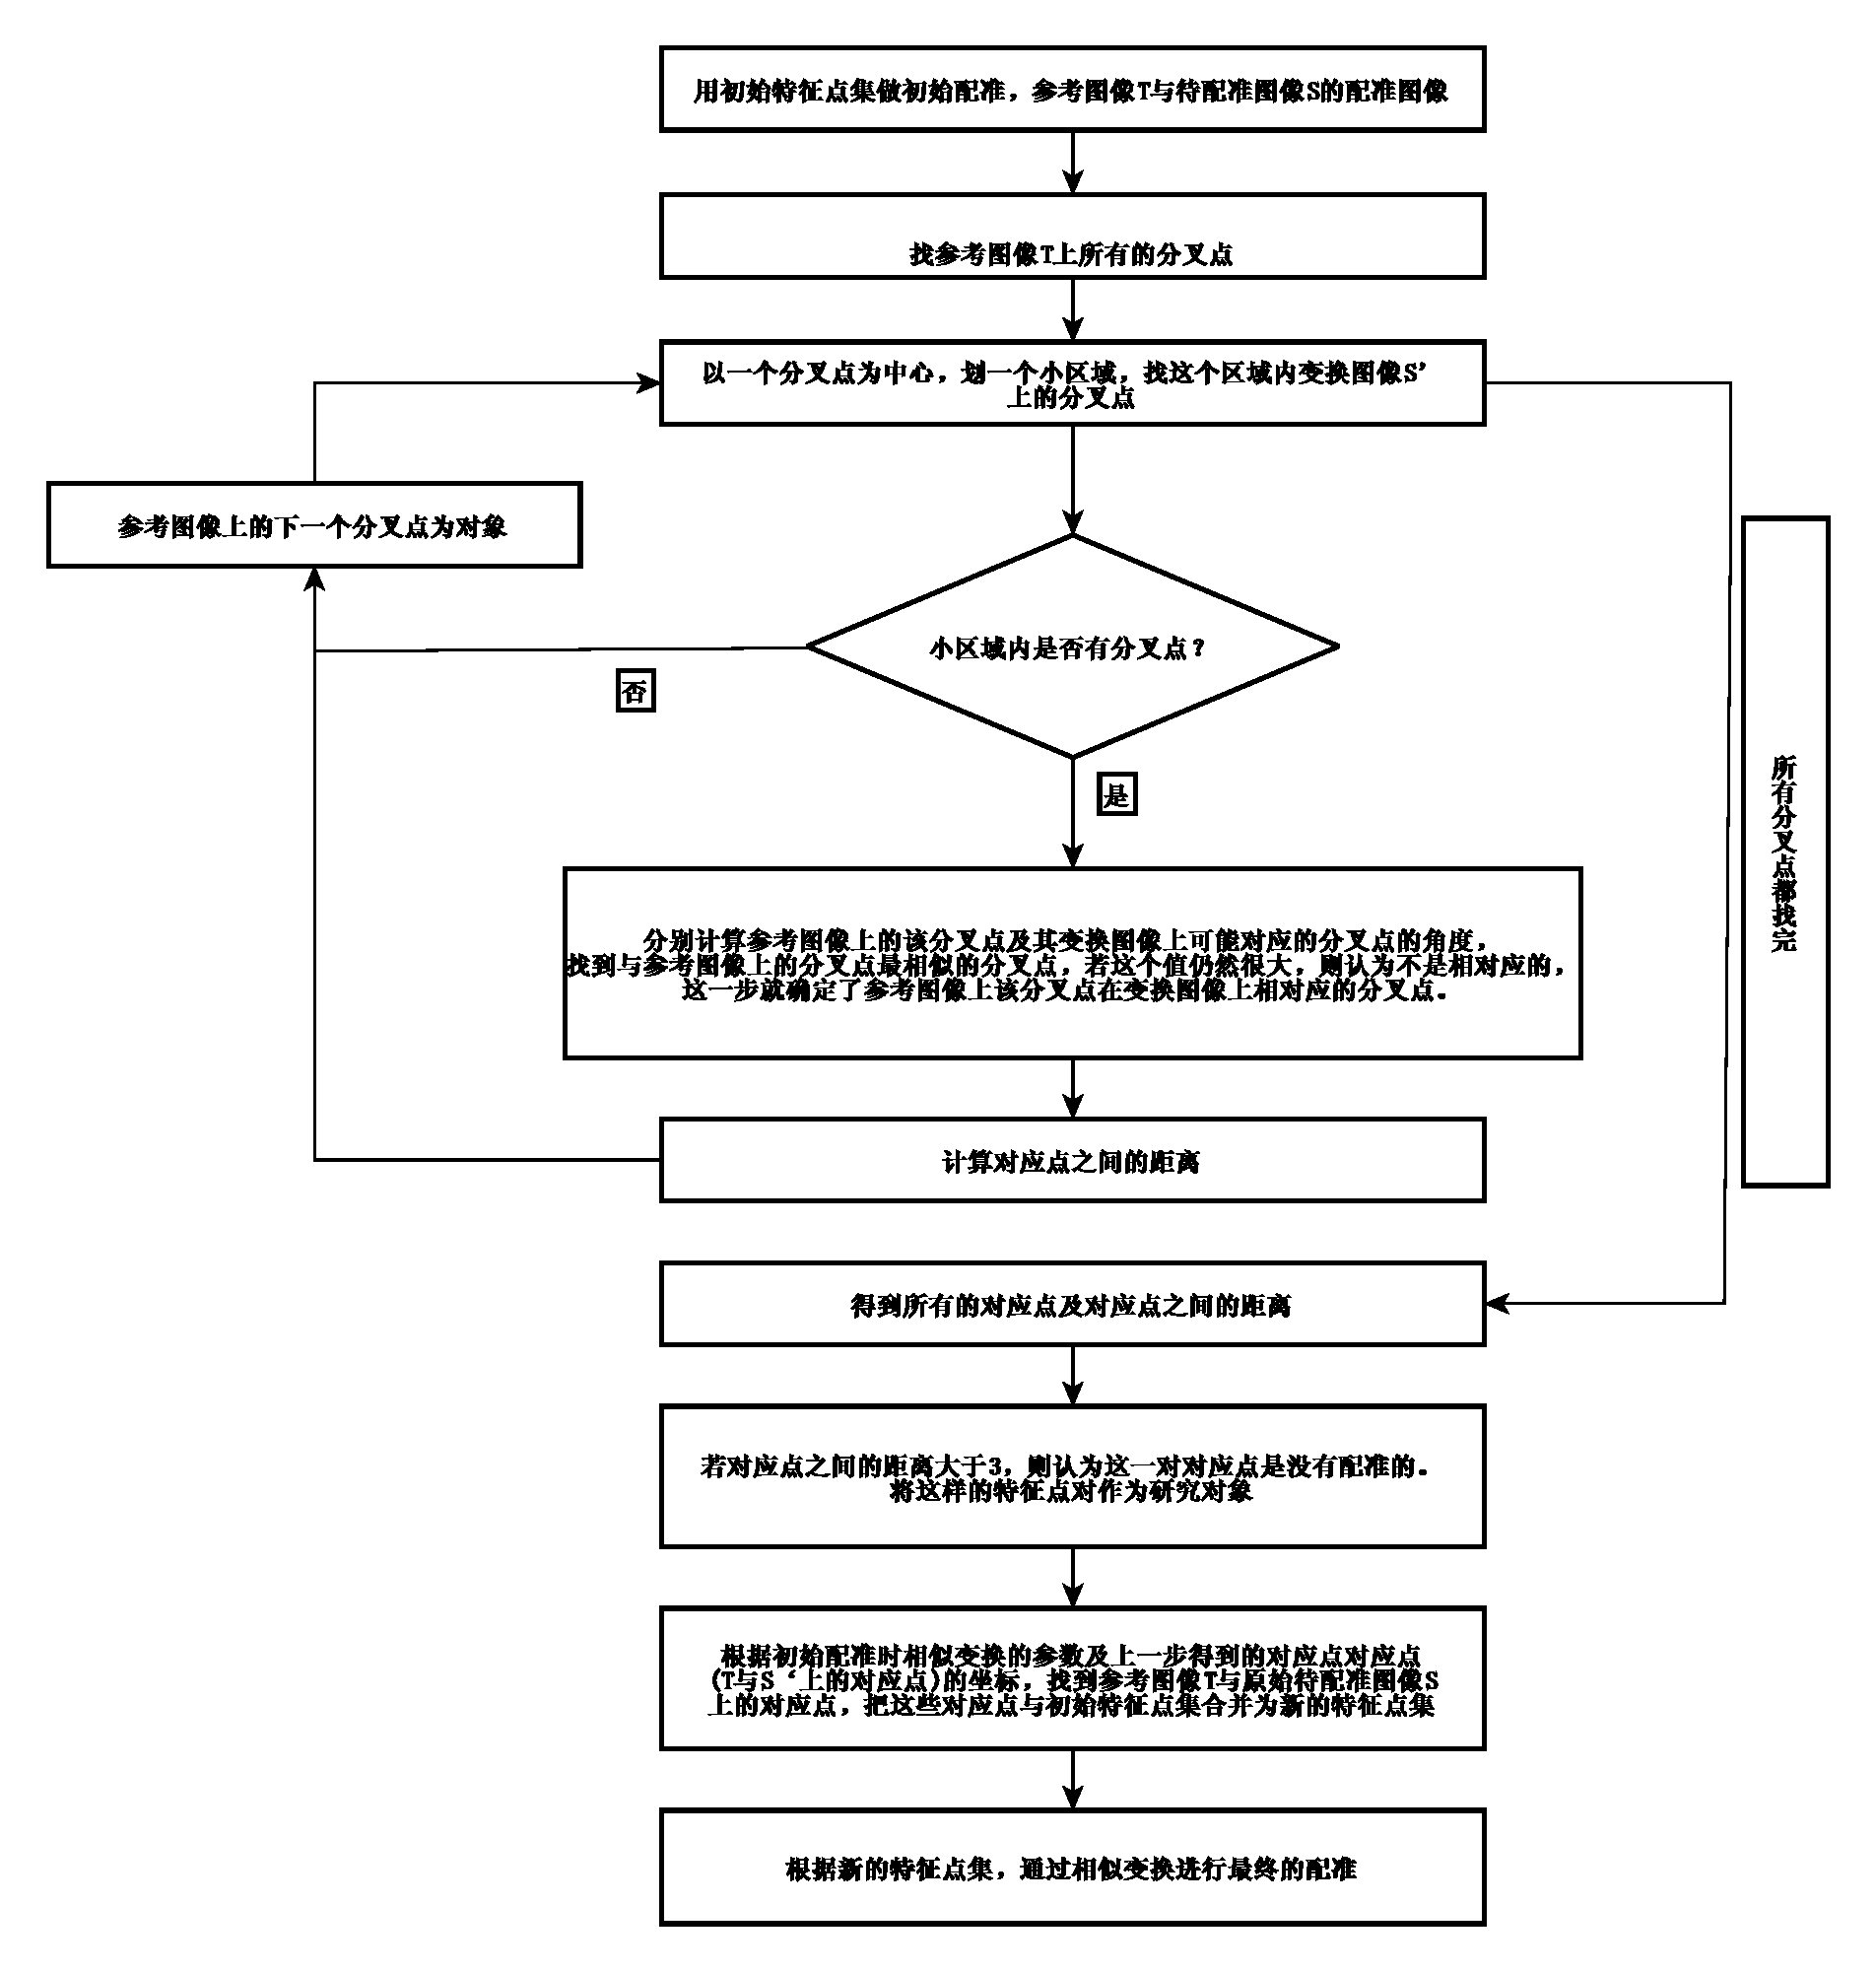
\includegraphics[width=1\textwidth]{figures/local}
  \caption{局部配准流程图}
  \label{fig:local}
\end{figure}

\begin{figure}[!ht]
\centering

\begin{minipage}[b]{0.3\textwidth} 
      \centering 
      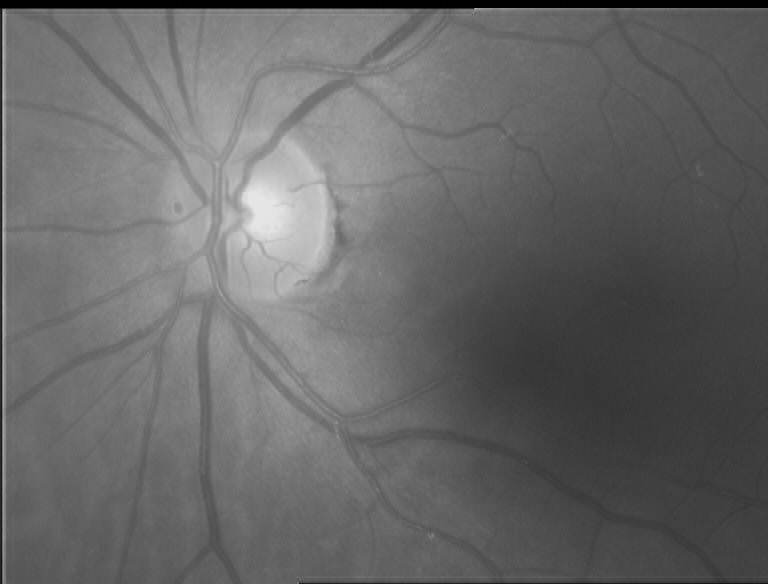
\includegraphics[width=4cm]{R160.png}
        \centerline{(a) 参考图像}\medskip
\end{minipage}
  \begin{minipage}[b]{0.3\textwidth}
    \centering
    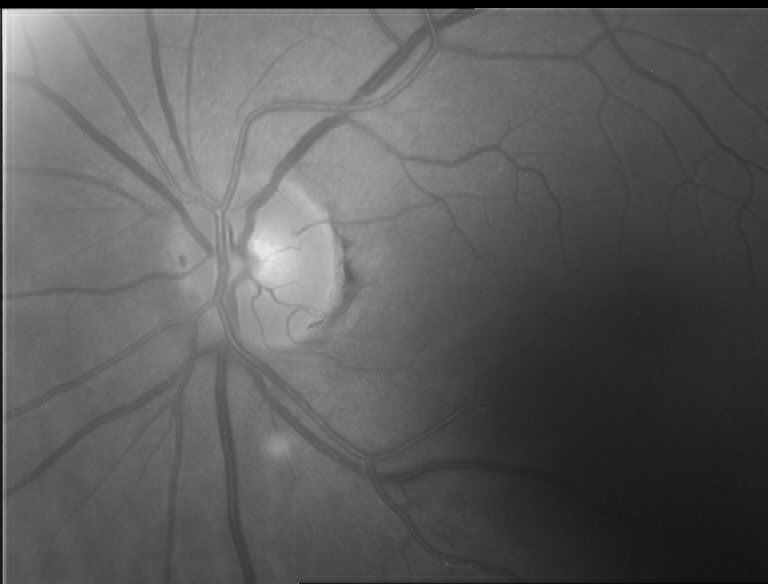
\includegraphics[width=4cm]{R161.png}
      \centerline{(b) 待配准图像}\medskip
  \end{minipage}
\begin{minipage}[b]{0.3\textwidth}
	\centering
      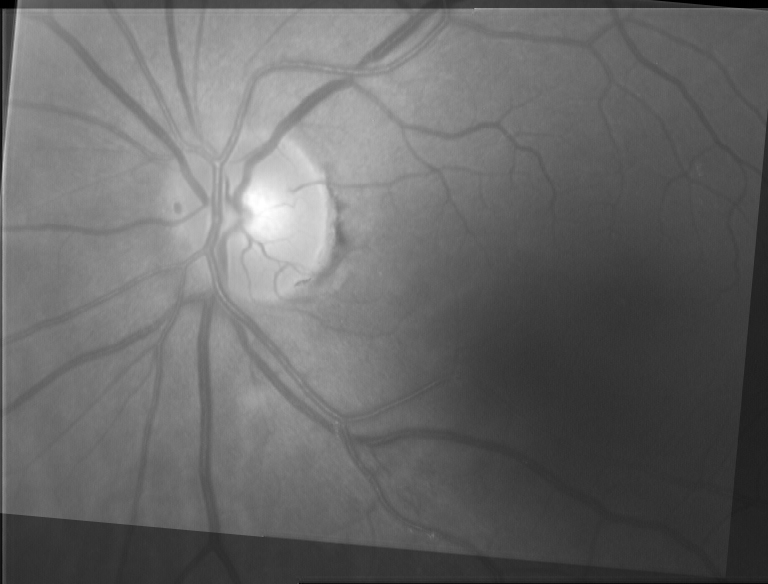
\includegraphics[width=4cm]{160-161-result.png}
        \centerline{(c) 配准后的原图像}\medskip
    \end{minipage}
\\
  \begin{minipage}[b]{0.48\textwidth}
    \centering
    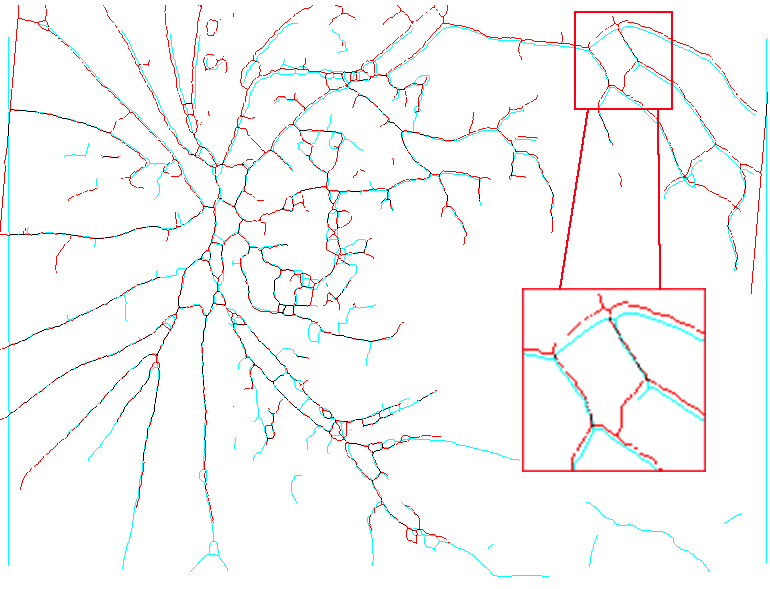
\includegraphics[width=5cm]{160-161-initial.png}
      \centerline{(d) 全局配准骨架化结果}\medskip
  \end{minipage}
 \begin{minipage}[b]{0.48\textwidth}
    \centering
      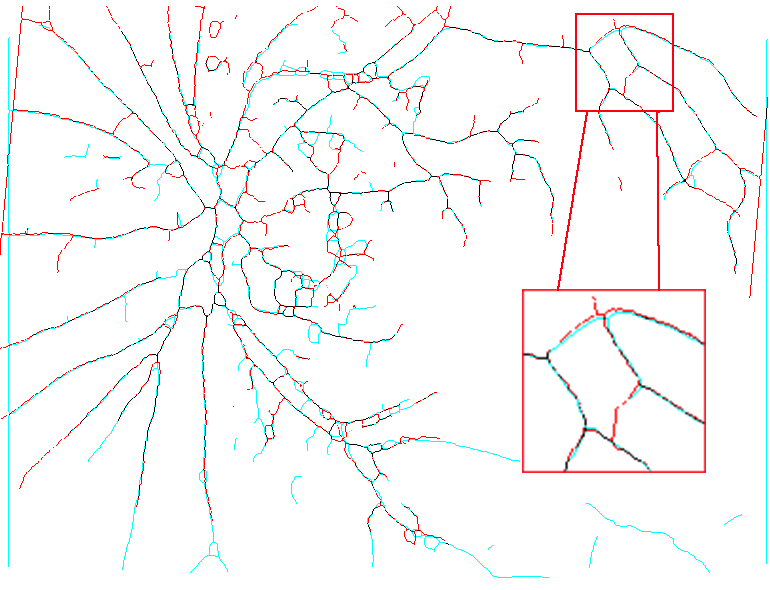
\includegraphics[width=5cm]{160-161-local.png}
        \centerline{(e) 局部配准骨架化结果}\medskip
    \end{minipage}
\\
  \begin{minipage}[b]{0.3\textwidth}
    \centering
    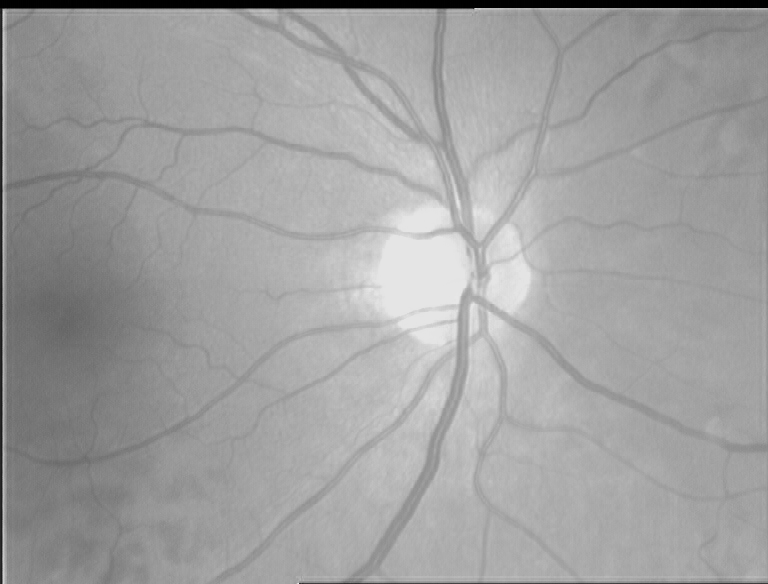
\includegraphics[width=4cm]{R096.png}
      \centerline{(f) 参考图像}\medskip
  \end{minipage}
\begin{minipage}[b]{0.3\textwidth}
      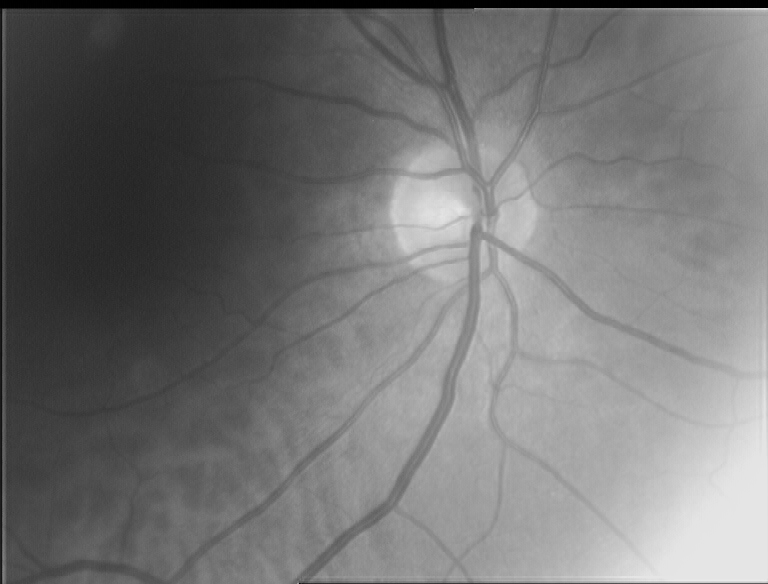
\includegraphics[width=4cm]{R212.png}
       \centerline{(g) 待配准图像}\medskip
    \end{minipage}
  \begin{minipage}[b]{0.3\textwidth}
    \centering
    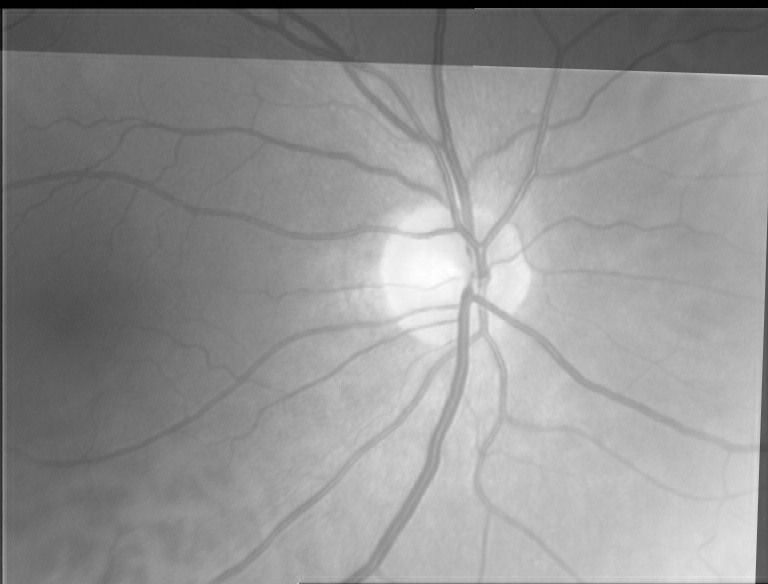
\includegraphics[width=4cm]{096-212-result.png}
          \centerline{(h) 配准后的原图像}\medskip
  \end{minipage}
\\
 \begin{minipage}[b]{0.48\textwidth}
    \centering
      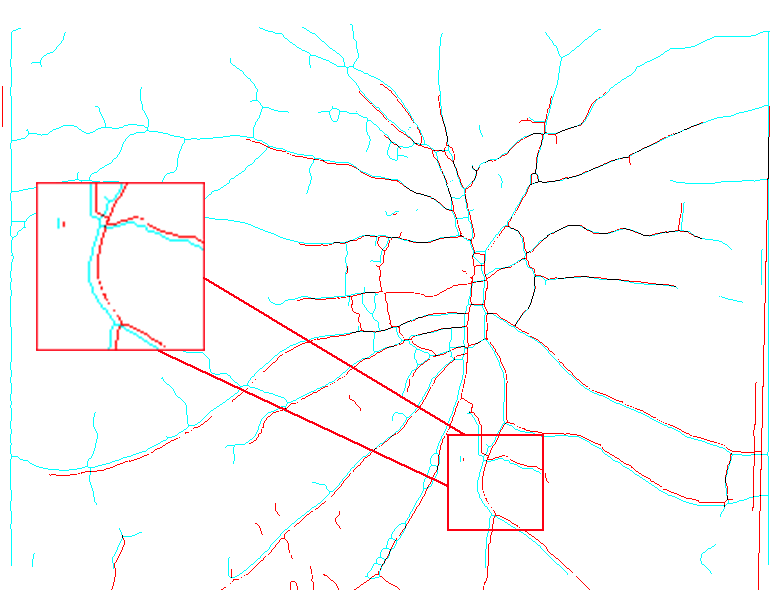
\includegraphics[width=5cm]{096-212-initial.png}
       \centerline{(i) 全局配准骨架化结果}\medskip
    \end{minipage}
  \begin{minipage}[b]{0.48\textwidth}
    \centering
    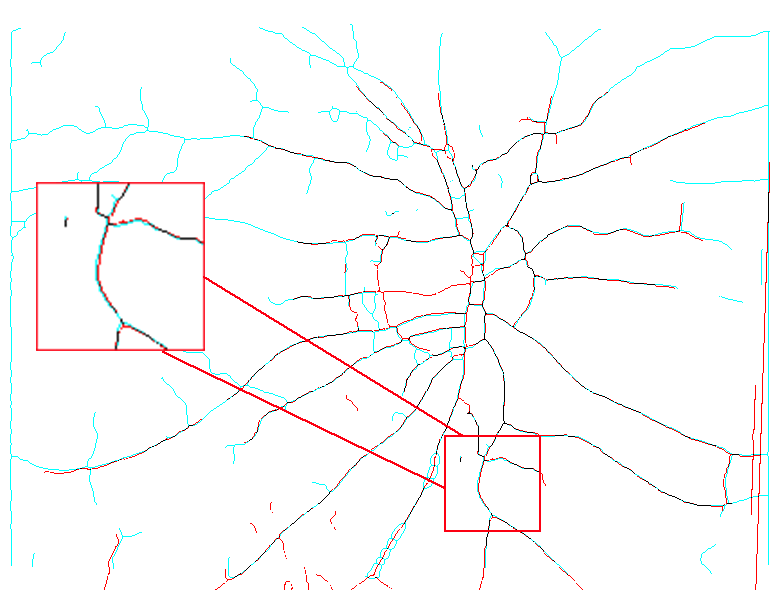
\includegraphics[width=5cm]{096-212-local.png}
           \centerline{(j) 局部配准骨架化结果}\medskip
  \end{minipage}
\caption{全局与局部配准结果}
\label{fig:final-results}
\end{figure}
\section{骨架化对准精度}

无论是对特定的图像、所使用的配准方法还是应用领域,都需要一个准确的评估方法来估计配准结果的准确性与精确性。精度评价是一个重要的问题,因为错误可能出现在配准过程的各个阶段有时很难区分配准错误和实际图像内容的差异。用人眼观察配准结果并不是一种十分科学的方法,因为存在一些主观因素来影响评估的准确性,通过定量的评价,可以得到对配准结果的准确估计。本节,我们介绍了几种基本的错误类型和评估方法\cite{barbara}并提出了我们自己的骨架化对准精度方法。


\begin{enumerate}
\item 定位误差。由于特征检测的不准确性引起的位移叫做定位误差。大多数特征检测的平均精度是真实的数据与计算机模拟的数据之间的比较,也可用于估计在特定情况下的定位误差。通过选择最优的特征检测算法,定位误差可能会减小,但在检测到的特征数量与平均定位误差之间通常有一个权衡。有时,我们更倾向于选择更多的特征和稍高的定位误差。

\item 匹配误差。匹配误差是在建立特征之间的对应关系时,错误匹配的特征数量。匹配误差是一个严重的问题,因为由于特征匹配错误,在用这对错误匹配的错误进行变换模型估计时,估计的变换参数是不准确的,因此通常会导致配准的失败。所以在进行特征匹配时应该尽量避免这个问题。幸运的是,在大多数情况下,匹配误差可以通过鲁棒性的匹配算法来避免。在两个不同的匹配方法应用于同一个特征集时,错误匹配可以通过一致性检验来发现。当两种方法都能找到的特征对为有效的特征对,其他的特征对需要做进一步的处理。若没有其他可靠的匹配方法,可以通过交叉验证的方式来消除错误的匹配。在每一步中,在特征集中排除一对特征并计算映射参数,然后观察通过这个模型,这对被排除的特征对的映射结果如何。若变换后与变换前的位移变化比较小,在某一阈值以下,则认为是有效的特征对。

\item 对准误差。对准误差为用于做配准的映射模型与实际的图像间的几何变形之间的差异。在实际应用中,对准误差是不可避免的。变换参数的计算可能不精确,导致所选择的映射模型可能与实际的变换模型的参数是不相对应的。

\end{enumerate}


然而,对准误差的计算是一项艰巨的任务,尤其对于生物医学应用,更加难以定量评估。因为缺乏标定好配准后的真实数据(Ground Truth),因此得到的配准后的图像不能与标定好的真实数据进行比较以得到估计结果。目前,有几种常用的评估方法,第一种方法是使用标记的位置信息,第二种是通过评估血管中心线的平均距离,第三种通过互信息\cite{kolar}。

\begin{enumerate}
\item 通过评估标记的位置,而已量化配准的精确性。配准前后的相应标记错误(ECL)的计算公式为:
\begin{align}
ECL^i = Median_{j}||p_j^i - T(q_j^i)|| 
\end{align}
其中,$p_j^i$和$q_j^i$是第i幅图像中的两个匹配的标记,T是最终的几何形变。中值对于标记对应的可能错误更具有鲁棒性。图像集的平均标记错误误差为每幅图像中值的平均值:
\begin{align}
E_1 = Mean_i(ECL^i)
\end{align}
\item 血管距离。血管距离准则值得是血管树中心线的平均距离。参考图像与待配准图像需进行分割及骨架化处理以得到血管中心线。但由于不同的图像的光照变化不同,分割结果也不同,为了克服这个问题,这种评价方法采用两幅图像的所有血管中心线点的中值距离作为标准。这对在分割中存在差异的情况具有鲁棒性。一对图像的中心线错误估计(CEM)可以定义为:
\begin{align}
CEM^i  = Median_j||p_j^i - T(q_j^i)||
\end{align}
其中,$p_j^i$和$q_j^i$是两对匹配的血管点,T是最终的几何形变。每对图像的中值都被计算后,求均值以得到数据集的最终配准估计:
\begin{align}
E_2 = Mean_i(CEM^i)
\end{align}
但CEM值取决于图像的分辨率。
\item 互信息可以作为配准结果的一个评估标准。归一化的互信息(NMI)可以通过计算图像重合区域来获得:
\begin{align}
NMI(A, B) = \frac{H(A)+H(B)}{H(A, B)}
\end{align}
$H(A), H(B)$和$H(A,B)$分别是边缘和联合熵。采用互信息进行评估的优点是它不依赖于图像的分辨率。
\end{enumerate}



我们采用多尺度分割方法,对于一幅参考图像与一幅待配准图像,分割与骨架化后会产生$14 \times 14$个多尺度结果,并且每一个尺度将产生7种环结构及其组合,故当这两幅图像进行配准时会产生$14 \times 14 \times 7$个配准结果。基于此,我们提出了一种骨架化对准精度用来定量的评估配准结果并且根据这个评估优化选择分割尺度与用来配准的环结构特征。

具体步骤为:
\begin{enumerate}
\item 给定一个参考图像的骨架化结果$M_i (i = 1, 2, \ldots, 14)$,一个待配准图像的骨架化结果$N_j (j = 1, 2, \ldots, 14)$,$N_j$与$M_i$用一种类型的环结构$L_k(k=1, 2, \ldots, 7)$在全局到局部的策略下进行配准,得到配准结果$N_{jMi}$。
\item 对于在$N_{jMi}$中的每个血管点,以这个血管点为中心,在$M_i$中选择一个$7 \times 7$区域,在这个区域中你计算与这个血管点相邻最近的像素的距离d。若在这个区域中没有与这个血管点相邻最近的点,则标记这个血管点无效。
\item 骨架化对准精度被定义为$SAEM_{ijk} = (\sum d) / Num_v$,$Num_v$是在$N_{jMi}$中无效点的数量。
\item 当$Num_v / Num_{N_j} \geq 50 \%$并且$Num_{N_{jMi}} / Num_{N_j} \geq 38 \%$时SAEM有效,$Num_{(.)}$表示在$(.)$中的像素数量。
\end{enumerate}

约束条件的设置是很有必要的,它可以排除一些配准结果偏差很大的情况。因为当两幅图像基本没有配准的情况下,在$7 \times 7$区域内可能检测不到相对应的血管点,这样会使得SAEM的值很小,相对应的图像则被认为是匹配的很精准。约束条件的设置就避免了这种情况的发生。通过骨架化对准精度,最佳的配准结果将会被自动的选择出来,而相对应的尺度和环结构的类型就会知晓。同时,SAEM算法还可以通过配准后两幅图像对应点的距离这个量化值来定量的评判配准结果。整个算法的整体框图如图\ref{fig:framework}。
\section{对比实验}
\label{}
据我们所知,目前没有公开的用来做视网膜配准的数据集。因此我们用VARIA数据集\cite{ortega2009retinal,ortega2009personal}来进行实验来评估我们的方法。VARIA数据集是用来做认证的,这个数据集目前包括从139个个体中获取的233张视网膜图像,其中有59组是从相同个体中拍摄的不同图像。从这59组数据中我们以每两张取自同一个体的不同视网膜图像为对象,共得到153对。这些视网膜图像是通过拓普康免散瞳NW-100相机在$768 \times 584$分辨率下获取的。

针对视网膜图像光照不均匀、中央亮、四周暗、反差过强、对比度弱、有强噪声干扰的特点,我们提出了基于环结构特征的从全局到局部的视网膜图像配准方法。环结构由血管分叉点和交叉点及与它们相连的血管组成。为了克服对视网膜分割结果的依赖性,我们采用多小波核多层分解方法,从而产生多尺度的血管树。不同尺度的血管树所代表的分割的精细程度不同。然后我们提出了基于空间的深度优先搜索算法来提取由多个不同数量的分叉点组成的多环特征,归一化的分支角度和长度来作为特征向量,采用相似性度量来进行全局初次配准。对于远离匹配特征的区域,我们采用局部分叉点信息来纠正配准精度。最后,我们采用骨架化对准精度来优化特征和尺度的选择,实验证明,我们的方法对于视网膜配准来说是有效且可行的。

为了通过实验来说明我们的方法是可行且有效的,我们通过不同变换模型、不同特征、不同方法进行了对比实验,用成功率(SR)及骨架化对准精度(SAEM)来定量的评估这153对图像的实验结果。

\subsection{不同变换模型之间的对比实验}

变换模型对于用来配准的不同特征是十分重要的。变换模型的选择能很大程度上影响配准结果。为了证明相似性变换更加适合环结构特征,我们用相似性变换、仿射变换、二次多项式变换进行了对比实验,表\ref{tab:models}给出了采用不同模型的配准结果。从表中可以看出,虽然多项式变换的SAEM值是最小的,但它对于环结构仍然是不适用的,因为其成功率只有16.99\%,所以不适用于做配准。仿射变换由于在变换过程中要改变环结构中的角度信息,所以配准成功率也相对较低。相似性变换对于我们提出的环结构特征是最适用的,成功率高达96.73\%,且SAEM值也相对较低。
\begin{table}[!ht]
\caption{不同变换模型之间的对比实验}
\centering
\begin{tabular}{lcc}
\toprule
变换模型 & SR  & SAEM (像素)\\
\midrule
相似性变换 & $\mathbf{96.73\%}$ & $\mathbf{0.938}$ \\
仿射变换 & $50.33\%$ & $1.010$              \\
二次多项式变换 & $16.99\%$ & $0.231$\\
\bottomrule
\end{tabular}
\label{tab:models}
\end{table}

图\ref{fig:transform-fig}给出了两组对比实验图,从图中可以看到相似性变换成功配准且配准精度较高,仿射变换基本配准,但有几个像素的距离,而多项式变换配准失败。
\begin{figure}[!ht]
\centering

\begin{minipage}[b]{0.48\textwidth} 
      \centering 
      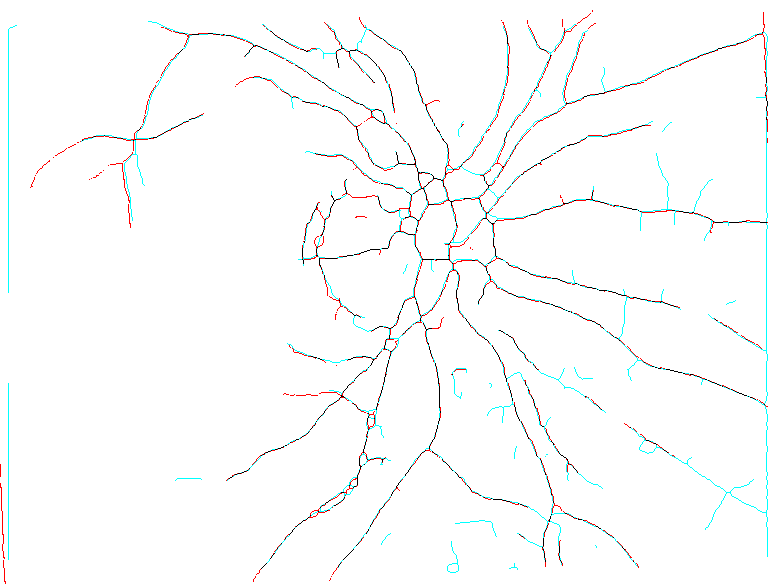
\includegraphics[width=6cm]{similarity1.png}
        \centerline{(a) 相似性变换}\medskip
\end{minipage}
  \begin{minipage}[b]{0.48\textwidth}
    \centering
    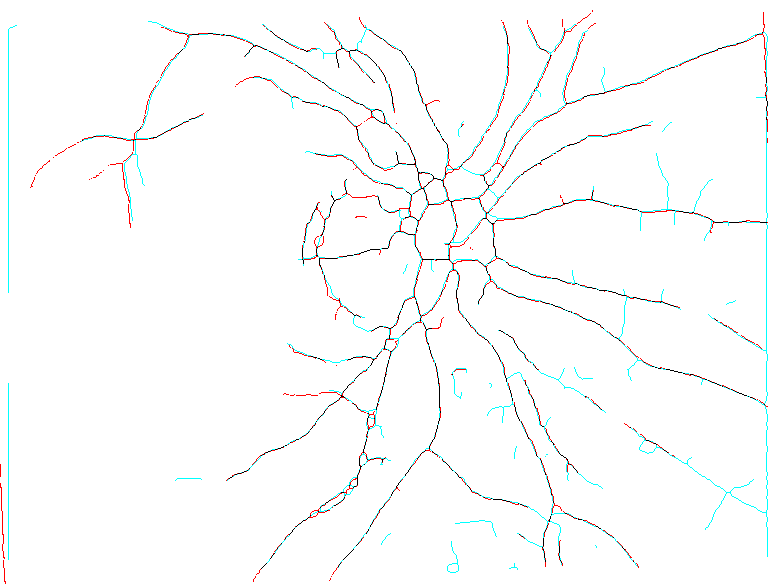
\includegraphics[width=6cm]{similarity2.png}
      \centerline{(d) 相似性变换变换}\medskip
  \end{minipage}
\\
  \begin{minipage}[b]{0.48\textwidth}
    \centering
    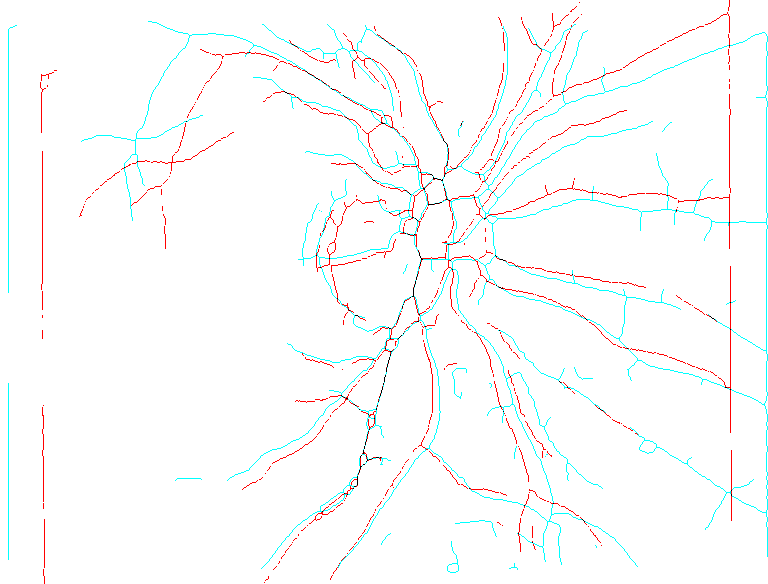
\includegraphics[width=6cm]{affine1.png}
      \centerline{(b) 仿射变换}\medskip
  \end{minipage}
 \begin{minipage}[b]{0.48\textwidth}
    \centering
      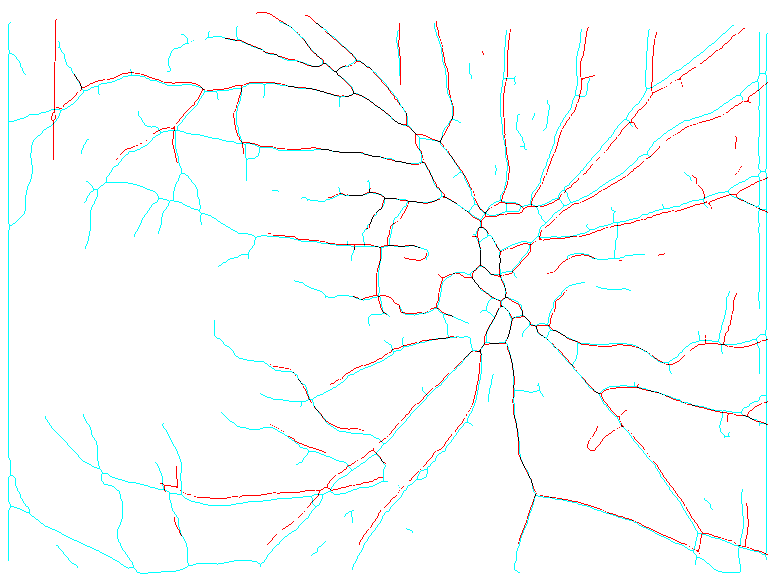
\includegraphics[width=6cm]{affine2.png}
        \centerline{(e) 仿射变换}\medskip
    \end{minipage}
\\
\begin{minipage}[b]{0.48\textwidth}
	\centering
      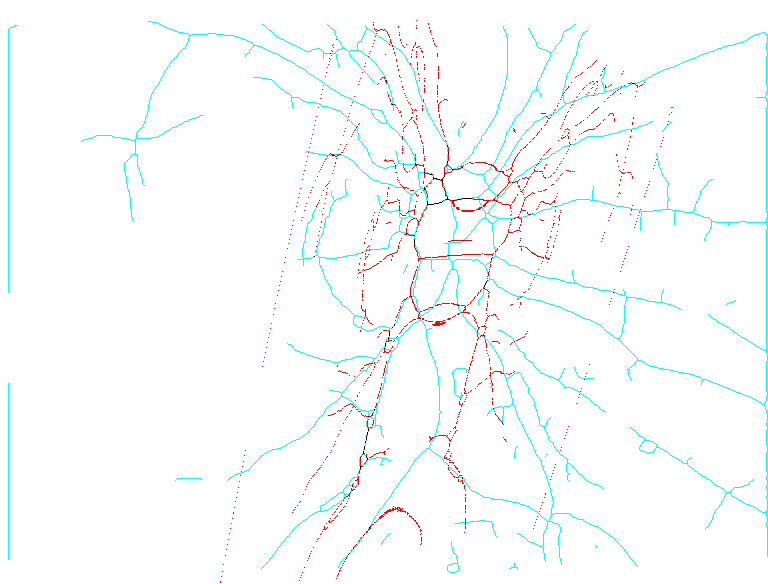
\includegraphics[width=6cm]{polynomial1.png}
        \centerline{(c) 二次多项式变换}\medskip
    \end{minipage}
  \begin{minipage}[b]{0.48\textwidth}
    \centering
    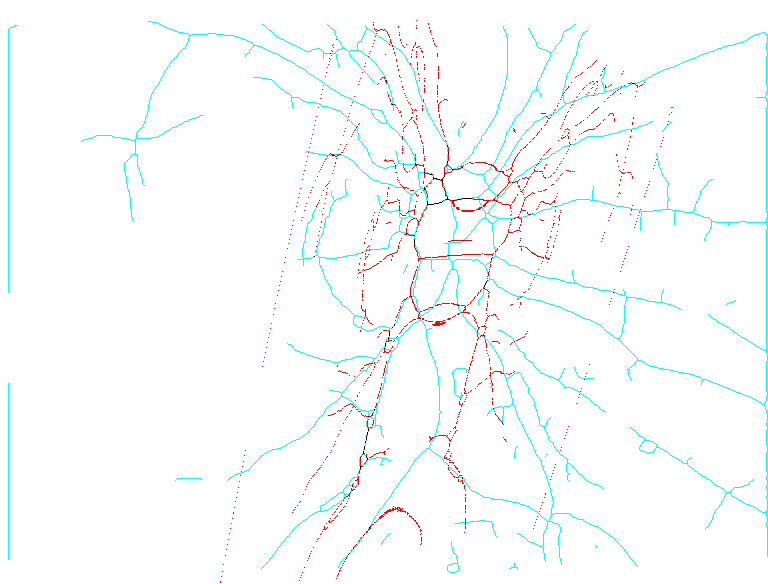
\includegraphics[width=6cm]{polynomial2.png}
      \centerline{(f) 二次多项式变换}\medskip
  \end{minipage}
\caption{不同变换模型的配准结果}
\label{fig:transform-fig}
\end{figure}

\subsection{不同特征之间的对比实验}

表\ref{tab:features}列出了采用不同特征的配准结果,即只用环上的点,环上的点及与环相连的血管上的点,环上的点、与环相连的血管上的点及局部分叉点三种情况。从表中我们可以明显看出,我们采用的从全局到局部的策略,即环+血管+分叉点的特征对配准来说更加鲁棒和准确,使得配准结果具有更高的准确率与最小的SAEM。

\begin{table}[!ht]
\caption{不同特征之间的对比实验}
\centering
\begin{tabular}{p{3.6cm}cc}
\toprule
特征 & SR  & SAEM (pixel)\\
\midrule
环 & $96.73\%$ & $0.938$\\
环 + 血管  & $97.39\%$ & $0.903$\\
环 + 血管 + 分叉点 & $\mathbf{100\%}$ & $\mathbf{0.879}$ \\
\bottomrule
\end{tabular}
\label{tab:features}
\end{table}

为了说明环结构更加适用于视网膜图像配准,我们也采用了Harrias角点检测算法与SIFT算法进行了特征提取,如图\ref{fig:ComparisionFeature}。Harrias角点检测算法检测到的特征点不能与实际观察的视网膜血管特征十分贴合,而且十分杂乱,很难找到对应关系,SIFT算法得到的匹配结果,匹配的特征点基本都是背景点而不是血管点,而且容易出现匹配错误。采用我们的算法,得到两对最匹配的环结构特征对,如图\ref{fig:ComparisionFeature}标记的红色及蓝色点。

\begin{figure}[!ht]
\centering
\begin{minipage}[b]{0.48\textwidth} 
      \centering 
      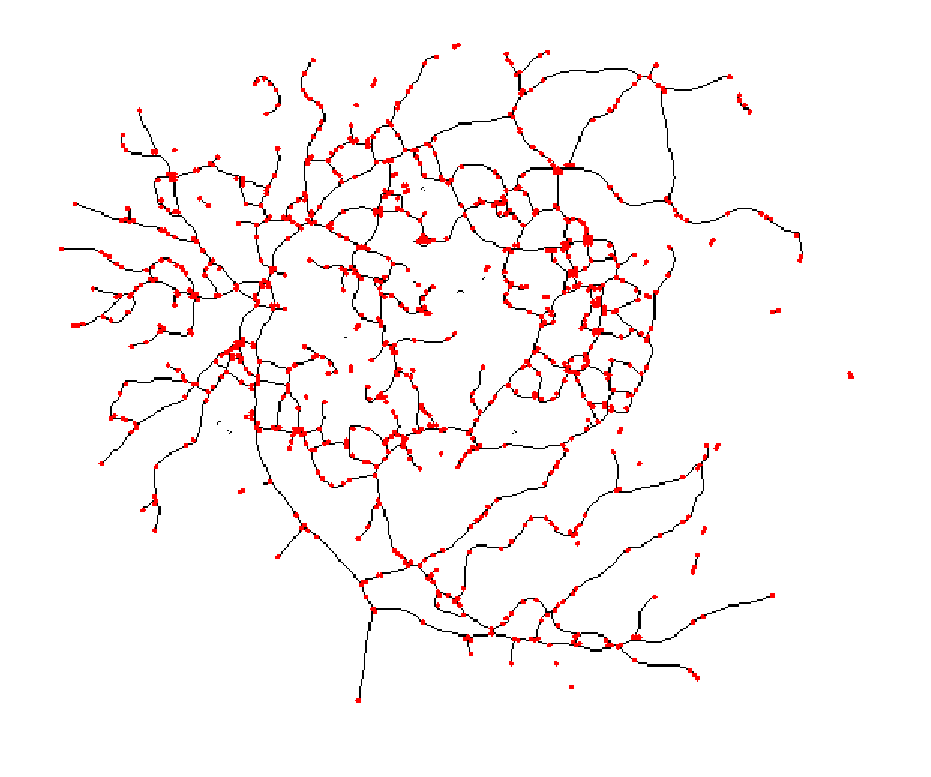
\includegraphics[width=7cm]{harrias1}
        \centerline{(a) 参考图像Harrias角点提取}\medskip
\end{minipage}
  \begin{minipage}[b]{0.48\textwidth}
    \centering
    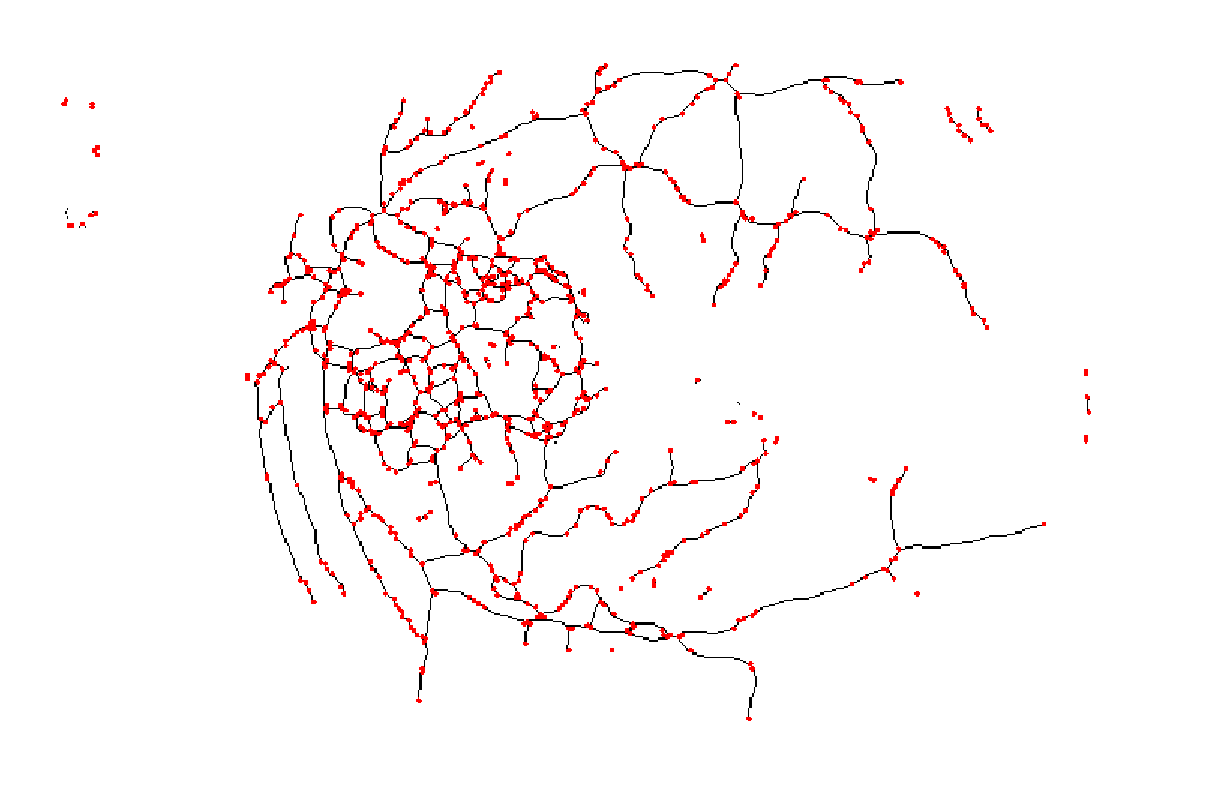
\includegraphics[width=8.5cm]{harrias2}
      \centerline{(b) 待配准图像Harrias角点提取}\medskip
  \end{minipage}
\begin{minipage}[b]{1\textwidth}
	\centering
      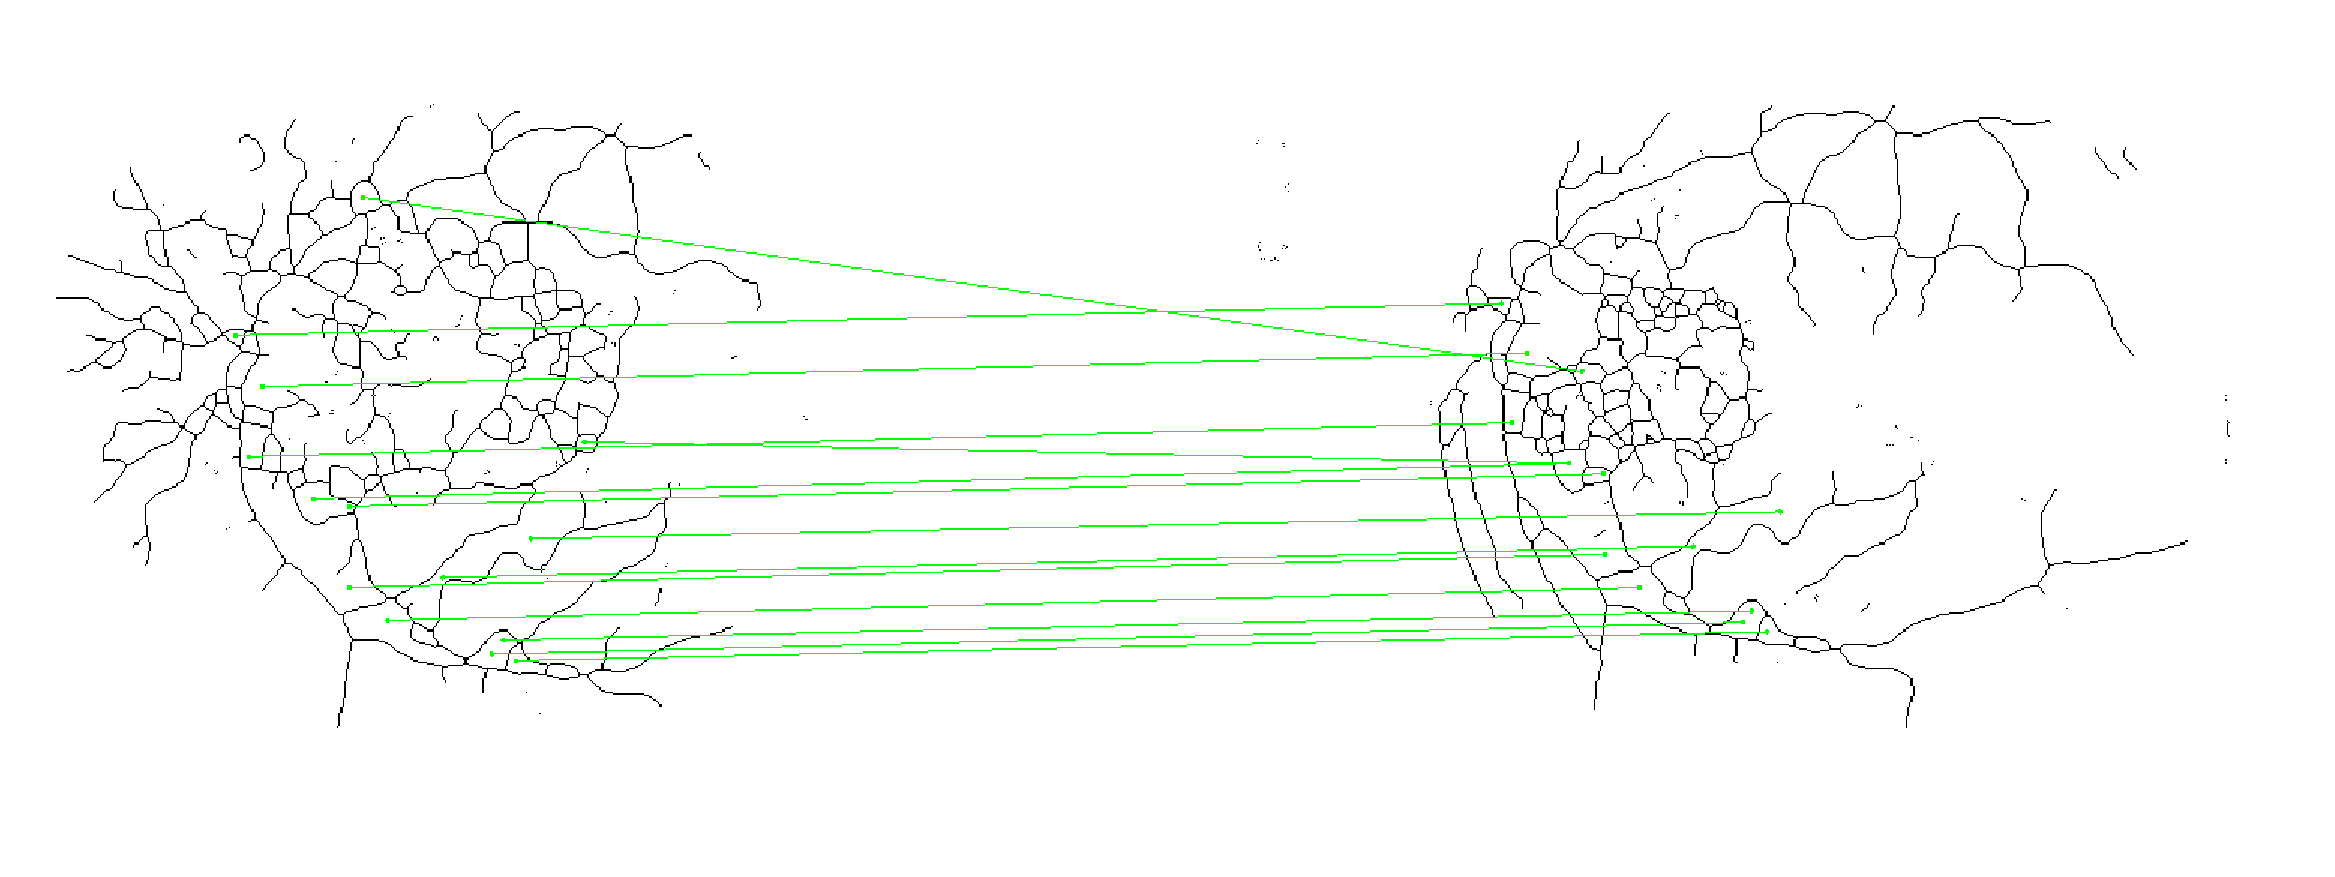
\includegraphics[width=15cm]{sift}
        \centerline{(c) SIFT特征匹配}\medskip
    \end{minipage}
\\
  \begin{minipage}[b]{0.48\textwidth}
    \centering
    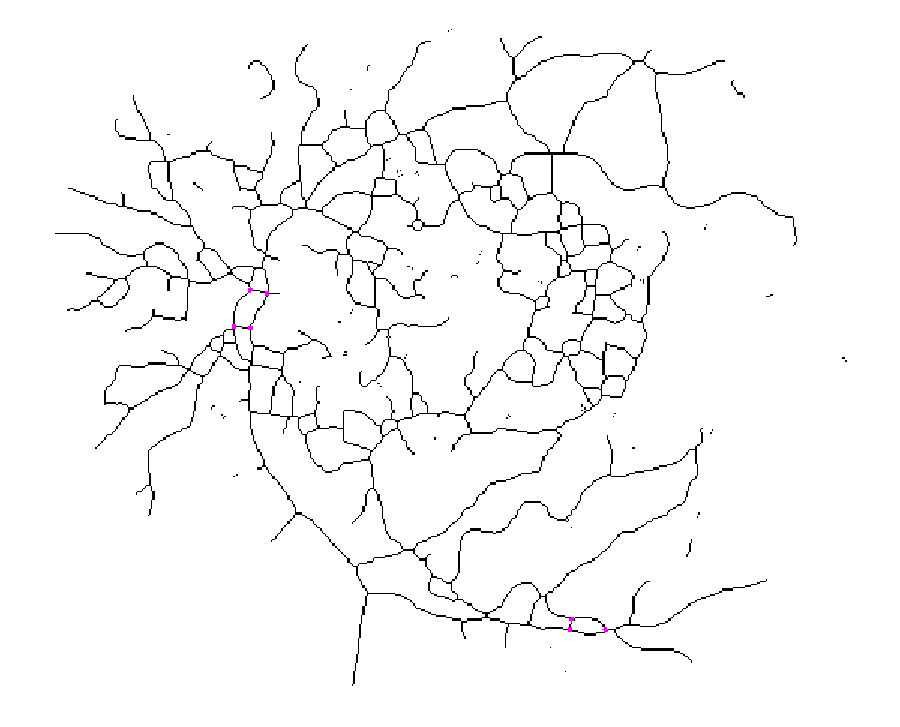
\includegraphics[width=7cm]{1}
      \centerline{(d) 参考图像中的环结构特征}\medskip
  \end{minipage}
 \begin{minipage}[b]{0.48\textwidth}
    \centering
      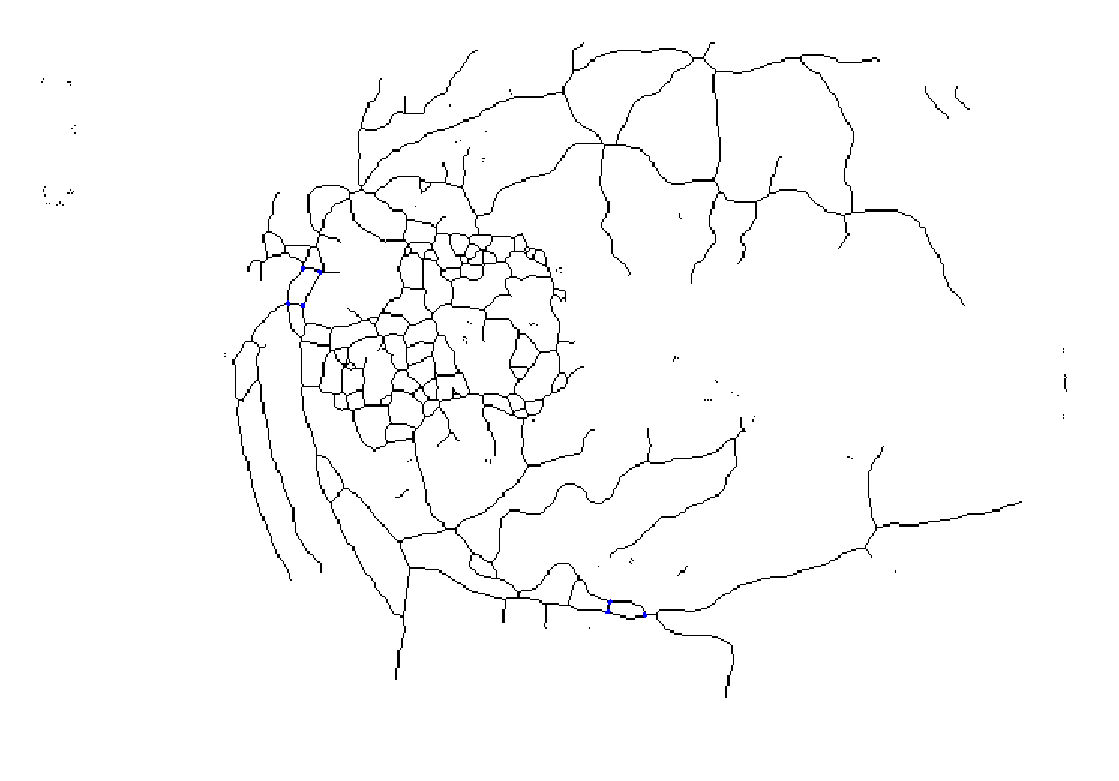
\includegraphics[width=8cm]{2}
        \centerline{(e) 待配准图像中的环结构特征}\medskip
    \end{minipage}
\caption{不同特征的配准结果}
\label{fig:ComparisionFeature}
\end{figure}


\subsection{不同方法之间的对比实验}

2011年,Chen\cite{chen2011retinal,chen2015retinal}等人结合视网膜图像的特点,提出了基于分叉结构的配准方法,分叉结构由一个主分叉点和与它相连的三个相邻分叉点组成,归一化的分支角度和长度作为特征向量,如图\ref{fig:bifurcation structure}。

\begin{figure}[!ht]
  \centering
  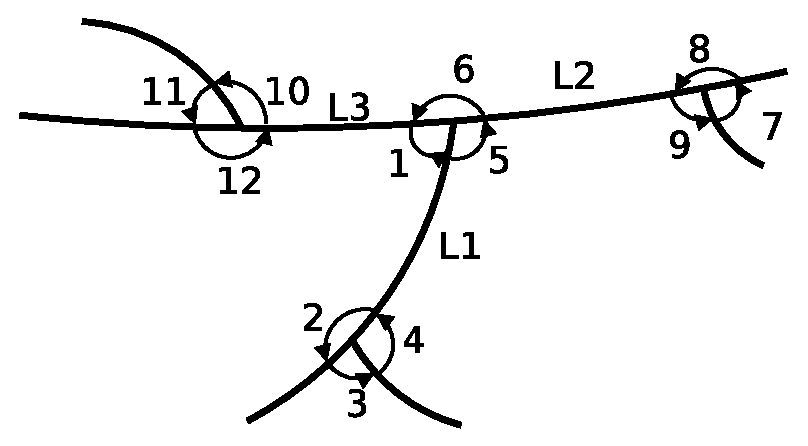
\includegraphics[width=0.4\textwidth]{bifurcation-structure}
  \caption{分叉结构特征}
  \label{fig:bifurcation structure}
\end{figure}

2013年,Shen\cite{shen2012blood}等人扩展了基于分叉结构的配准方法,利用局部的精细配准来纠正配准精度。其局部配准的主要步骤是:
\begin{enumerate}
\item 分别在参考图像和变换后图像上检测分叉点并进行坐标比对,利用界定盒原理找到未匹配上的分叉点。
\item 在参考图像上以任一分叉点q为中心,划定一个$M / p \times N / P$大小的区域,其中P是一个固定值,$M \times N$为图像大小,假如在这个区域内有K个分叉点未匹配上,则说明这个区域的配准精度不高,需要再次进行局部配准。
\item 在未精准配准区域中与参考图像中找到一组对应的分叉结构,得到组成分叉结构的分叉点的坐标。这对分叉结构能使得相似性度量最小,即是最匹配的分叉结构。
\item 将局部区域内提取的配对分叉点与初次配准时的分叉结构上的分叉点结合,利用仿射变换再次配准,得到最终配准结果。
\end{enumerate}

为了说明环结构更加鲁棒和稳定,我们通过实验与上述两种方法进行了对比,结果如表\ref{tab:methods}。从表中可以看到,我们的方法能达到100\%的准确率且SAEM值也相比其他两种方法小,说明我们的方法更加适用于视网膜图像配准。

\begin{table}[!ht]
\caption{不同的方法之间的对比实验}
\centering
\begin{tabular}{lcc}
\toprule
Methods & SR & SAEM (pixel)\\
\midrule
分叉结构 & $52.9\%$ & $1.009$\\
分叉结构 + 局部特征& $60.13\%$ & $0.978$\\
我们的方法 & $\mathbf{100\%}$ & $\mathbf{0.879}$\\
\bottomrule
\end{tabular}
\label{tab:methods}
\end{table}
图\ref{fig:methods-fig}给出了两组不同方法之间的对比实验图像。从图中可以看到,采用分叉结构特征时总有几个像素的偏差,配准精度不高,而加上了局部特征后配准得到了纠正,但精度仍不如我们的方法高。
\begin{figure}[!ht]
\centering
\begin{minipage}[b]{0.48\textwidth} 
      \centering 
      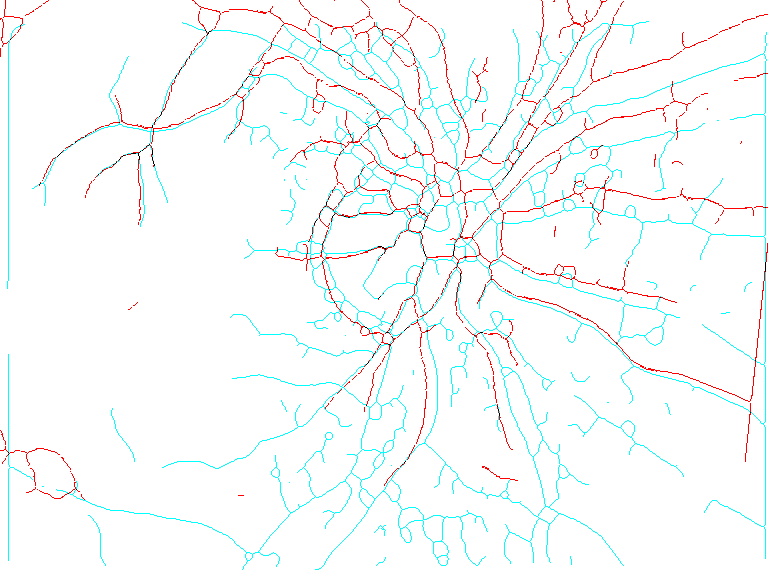
\includegraphics[width=6cm]{bifu1.png}
        \centerline{(a) 分叉结构特征}\medskip
\end{minipage}
  \begin{minipage}[b]{0.48\textwidth}
    \centering
    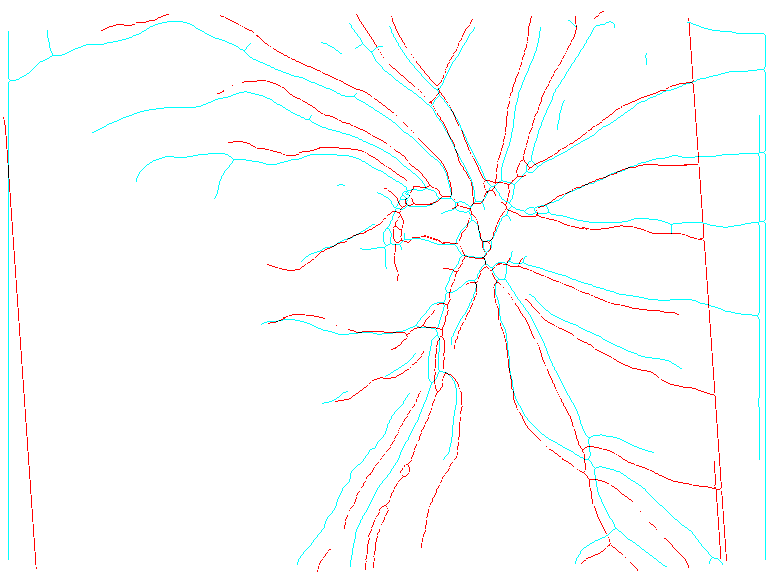
\includegraphics[width=6cm]{bifu2.png}
      \centerline{(d) 分叉结构特征}\medskip
  \end{minipage}
  \begin{minipage}[b]{0.48\textwidth}
    \centering
    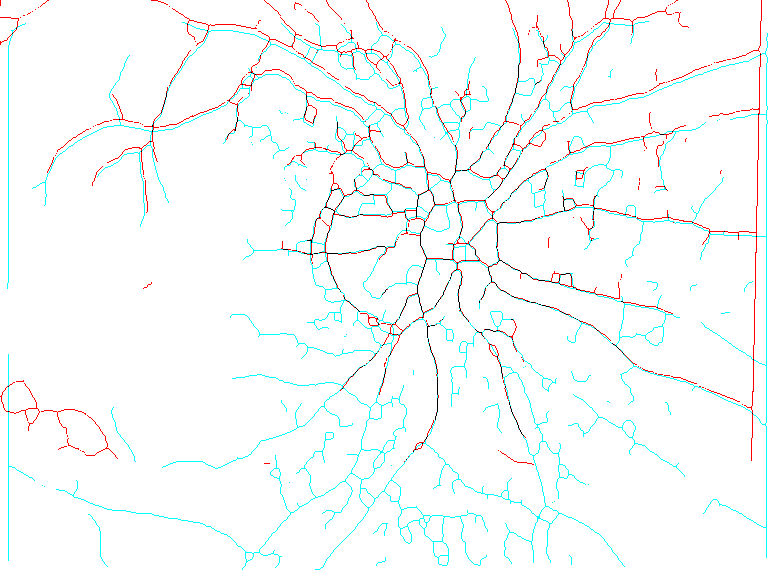
\includegraphics[width=6cm]{bifu-local1.png}
      \centerline{(b) 分叉结构 + 局部特征}\medskip
  \end{minipage}
 \begin{minipage}[b]{0.48\textwidth}
    \centering
      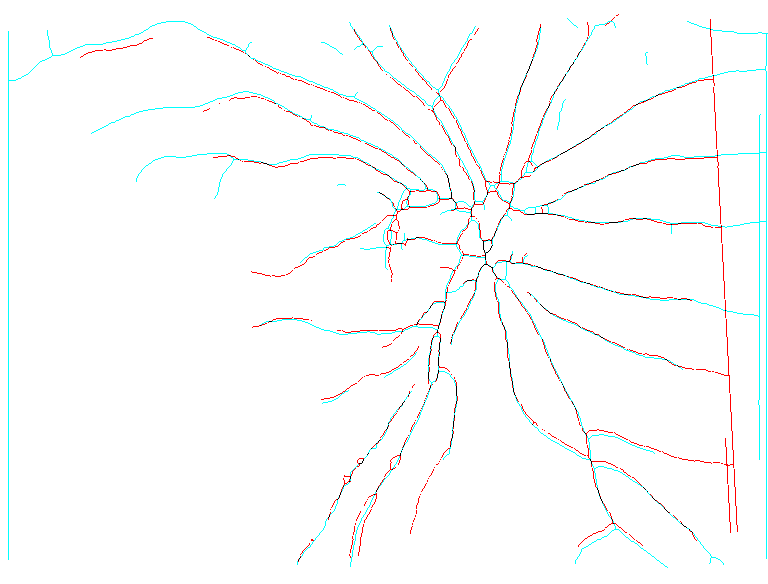
\includegraphics[width=6cm]{bifu-local2.png}
        \centerline{(e) 分叉结构 + 局部特征}\medskip
    \end{minipage}
\begin{minipage}[b]{0.48\textwidth}
	\centering
      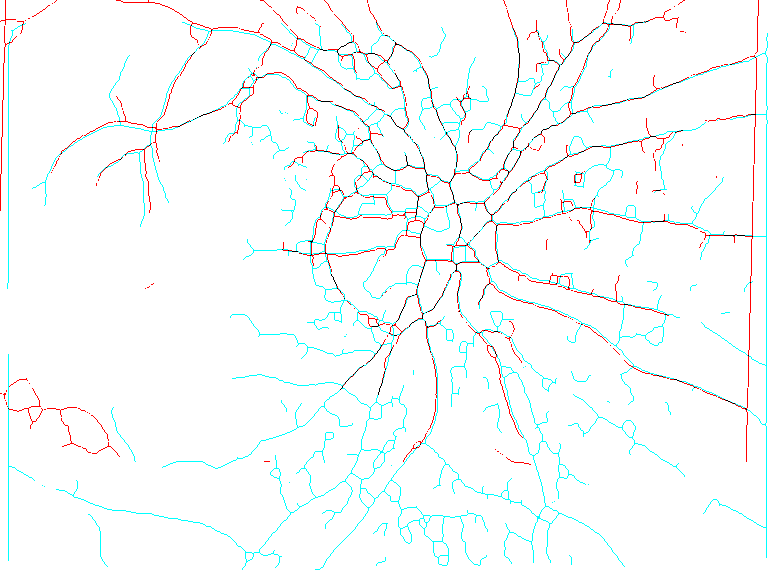
\includegraphics[width=6cm]{ours1.png}
        \centerline{(c) 我们的方法}\medskip
    \end{minipage}
  \begin{minipage}[b]{0.48\textwidth}
    \centering
    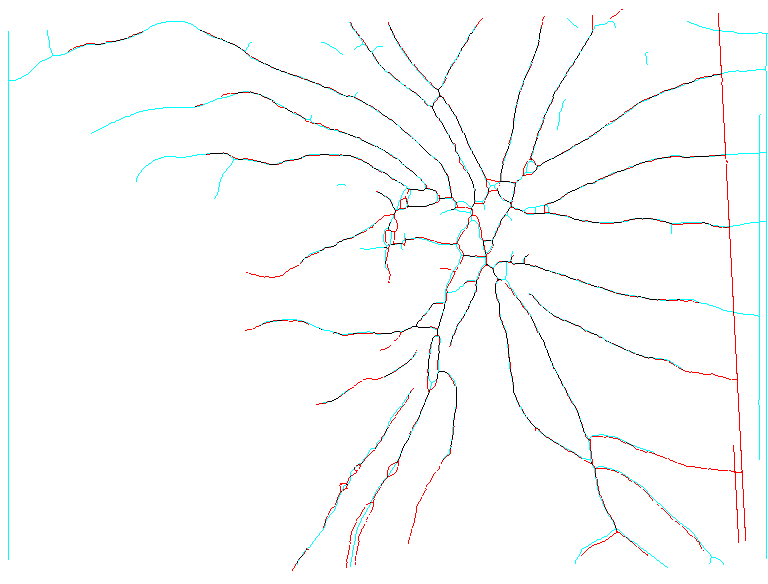
\includegraphics[width=6cm]{ours2.png}
      \centerline{(f) 我们的方法}\medskip
  \end{minipage}
\caption{不同方法的配准结果}
\label{fig:methods-fig}
\end{figure}

\section{本章小节}
\label{}

视网膜配准技术是分析与诊断眼科疾病的关键技术。基于特征的视网膜配准通常采用鲁棒的视网膜特征来进行配准,故而相对于基于强度的方法更加有效。我们提出了一种采用多尺度及多环特征的从全局到局部的视网膜配准技术。多尺度血管图像通过多小波核及多层分解分割方法得到,尺度越大,分割出的血管就越精细。多环特征是不同种类的环结构的组合。环结构是由血管分叉点或相交点及它们之间的血管组成,是由我们提出的动态路径移动算法检测出的。环特征结构通过归一化的分支角度与分支长度描述为特征向量,通过采用相似性度量准则,找到最匹配的环特征。组成环结构的血管分叉点及与环结构相连的血管上的点组成初始特征点集,采用相似性变换得到全局初始配准结果。为了优化配准结果,我们通过检测局部未配准的分叉点,加入特征点集来进行二次局部配准,从而保证了配准精度。骨架化对准精度用来选择最佳配准结果并进行定量的评估。通过实验证明,我们的方法对视网膜配准是可行且有效的。
